%%% Exemplo de utilização da classe ITA
%%%
%%%   por        Fábio Fagundes Silveira   -  ffs [at] ita [dot] br
%%%              Benedito C. O. Maciel     -  bcmaciel [at] ita [dot] br
%%%              Giovani Volnei Meinertz   -  giovani [at] ita [dot] br
%%%    	         Hudson Alberto Bode       -  bode [at] ita [dot]br
%%%    	         P. I. Braga de Queiroz    -  pi [at] ita [dot] br
%%%    	         Jorge A. B. Gripp         -  gripp [at] ita [dot] br
%%%    	         Juliano Monte-Mor         -  jamontemor [at] yahoo [dot] com [dot] br
%%%    	         Tarcisio A. B. Gripp      -  tarcisio.gripp [at] gmail [dot] com
%%%
%%%   Versão para overleaf:
%%%   por        Alejandro A. Rios Cruz    - aarc.88@gmail.com
%%%              Saulo Gómez               - sagomezs@unal.edu.co
%%%              Ocimar Santos             - ocimar.acad@gmail.com
%%%
%%%   Template disponibilizado em:
%%%              Overleaf: https://pt.overleaf.com/latex/templates/thesis-template-aeronautics-institute-of-technology-ita/yhfrqqydpygk
%%%
%%%   Contribuia você também!
%%%              GitHub:   https://github.com/AlejandroRios/Template_Thesis_ITA
%%%
%%%  IMPORTANTE: O texto contido neste exemplo nao significa absolutamente nada.  :-)
%%%              O intuito aqui eh demonstrar os comandos criados na classe e suas
%%%              respectivas utilizacoes.
%%%
%%%  Tese.tex  2016-08-25
%%%  $HeadURL: http://www.apgita.org.br/apgita/teses-e-latex.php $
%%%
%%% ITALUS
%%% Instituto Tecnológico de Aeronáutica --- ITA, Sao Jose dos Campos, Brasil
%%%                   http://groups.yahoo.com/group/italus/
%%% Discussion list: italus {at} yahoogroups.com
%%%
%++++++++++++++++++++++++++++++++++++++++++++++++++++++++++++++++++++++++++++++
% Para alterar o TIPO DE DOCUMENTO, preencher a linha abaixo \documentclass[?]{?}
%   \documentclass[tg]{ita}			= Trabalho de Graduacao
%   \documentclass[tgfem]{ita}	= Para Engenheiras
%   								msc     		= Dissertacao de Mestrado
%   								mscfem   		= Para Mestras
%   								dsc      		= Tese de Doutorado
%   								dscfem   		= Para Doutoras
%   								quali    		= Exame de Qualificacao
%   								qualifem 		= Exame de Qualificacao para Doutoras
% Para 'Draft Version'/'Versao Preliminar' com data no rodape, adicionar 'dv':
%   \documentclass[dsc, dv]{ita}
% Para trabalhos em Inglês, adicionar 'eng':
%   \documentclass[dsc, eng]{ita}
%		\documentclass[dsc, eng, dv]{ita}
%++++++++++++++++++++++++++++++++++++++++++++++++++++++++++++++++++++++++++++++
\documentclass[tg]{ita}    % ITA.cls based on standard book.cls
% Quando alterar a classe, por exemplo de [msc] para [msc, eng]) rode mais uma vez o botão BUILD OUTPUT caso haja erro
\usepackage[utf8]{inputenc}
\usepackage{ae}
\usepackage{graphicx}
\usepackage{epsfig}
\usepackage{amsmath}
\usepackage{amssymb}
\usepackage{subcaption}
\usepackage{multirow}
\usepackage{float}
\usepackage{amsthm}
\usepackage{url}         % formats URL addresses properly
\usepackage{appendix}    % allows appendix section to be included
\usepackage{lscape}      % allows a page to be rendered in landscape mode
\usepackage{multicol}    % allows text in multi columns
\usepackage{cancel}      % needed to show canceled terms in equations
\usepackage{lettrine}
\usepackage{float}
\usepackage{placeins}


%HHHHHHHHHHHHHHHHHHHHHHHHHHHHHHHHHHHHHHHHHHHHHHHHHHHHHHHHHHHHHHHHHHHHHHHHHHHHHHHHHHHHHHHHHHHHHHHHHHHHHHHHHHHH
%\usepackage{subfigure}
%\usepackage{subfigmat}
%PACOTEFIGURAS_SE _ERRADO_ESXCLUIR_ACIMA
\usepackage{booktabs}
%PACOTETABELAS_SE _ERRADO_ESXCLUIR_ACIMA
%HHHHHHHHHHHHHHHHHHHHHHHHHHHHHHHHHHHHHHHHHHHHHHHHHHHHHHHHHHHHHHHHHHHHHHHHHHHHHHHHHHHHHHHHHHHHHHHHHHHHHHHHHHHH

%++++++++++++++++++++++++++++++++++++++++++++++++++++++++++++++++++++++++++++++
% Espaçamento padrão de todo o documento
%++++++++++++++++++++++++++++++++++++++++++++++++++++++++++++++++++++++++++++++
\onehalfspacing

%singlespacing Para um espaçamento simples
%onehalfspacing Para um espaçamento de 1,5
%doublespacing Para um espaçamento duplo

%++++++++++++++++++++++++++++++++++++++++++++++++++++++++++++++++++++++++++++++
% Identificacoes (se o trabalho for em inglês, insira os dados em inglês)
% Para entradas abreviadas de Professora (Profa.) em português escreva: Prof$^\textnormal{a}$.
%++++++++++++++++++++++++++++++++++++++++++++++++++++++++++++++++++++++++++++++
\course{Engenheria Aeroespacial}  % Programa de PG ou Curso de Graduação
%\area{Aircraft Design} % Área de concentração na PG (Não utilizado no caso de TG)

% Autor do trabalho: Nome Sobrenome
\authorgender{masc}                     %sexo: masc ou fem
\author{Pedro Kuntz}{Puglia}
\itaauthoraddress{Rua H8C, Ap. 303}{12.228- 462}{São José dos Campos- SP}

% Titulo da Tese/Dissertação
\title{Caracterização de sistema de propulsão a gás frio com empuxo vetorial}

% Orientador
\advisorgender{masc}                    % masc ou fem
\advisor{Prof.~Dr.}{Leonardo Gouvêa}{ITA}

% Coorientador (Caso não haja coorientador, colocar ambas as variáveis \coadvisorgender e \coadvisor comentadas, com um % na frente)
% \coadvisorgender{fem}									% masc ou fem
% \coadvisor{Prof$^\textnormal{a}$.~Dr$^\textnormal{a}$.}{Doralice Serra}{OVNI}

% Pró-reitor da Pós-graduação
% \bossgender{masc}												% masc ou fem
% \boss{Prof.~Dr.}{John von Neumann}

%Coordenador do curso no caso de TG
\bosscoursegender{fem}									% masc ou fem
\bosscourse{Profa.~Dra.}{Cristiane Martins}

% Palavras-Chaves informadas pela Biblioteca -> utilizada na CIP
\kwcip{Propulsão}
\kwcip{Empuxo Vetorial}
\kwcip{Gás Frio}

% membros da banca examinadora

% \examiner{Prof. Dr.}{Alan Turing}{Presidente}{ITA}
% \examiner{Prof. Dr.}{Linus Torwald}{}{UXXX}
% \examiner{Prof. Dr.}{Richard Stallman}{}{UYYY}
% \examiner{Prof. Dr.}{Donald Duck}{}{DYSNEY}
% \examiner{Prof. Dr.}{Mickey Mouse}{}{DISNEY}

% Data da defesa (mês em maiúsculo, se trabalho em inglês, e minúsculo se trabalho em português)
\date{23}{novembro}{2022}

% Número CDU - (somente para TG)
\cdu{???.??}

% Glossario
\makeglossary
\frontmatter

\begin{document}
%%%%%%%%%%%%%%%%%%%%%%%%%%%%%%%%%%%%%%%%%
%%% - - Modelo para relatório ITA - - %%%
%%%%%%%%%%%%%%%%%%%%%%%%%%%%%%%%%%%%%%%%%
%%%    Documente as mudanças e os     %%%
%%%       upgrades na estrutura       %%%
%%%%%%%%%%%%%%%%%%%%%%%%%%%%%%%%%%%%%%%%%

\documentclass[12pt, a4paper]{article}

% Fonte e símbolos
% \usepackage{fontspec}
% \setmainfont{Times New Roman}
\usepackage[brazilian]{babel}
% Tamanho padrão da folha
\usepackage[left=1.5cm,right=1.5cm,top=1.5cm,bottom=1.5cm]{geometry}
\usepackage{csquotes}
\usepackage{latexsym}
\usepackage{amsmath}
\usepackage{textcomp}
\usepackage{gensymb}
\usepackage{indentfirst}
\usepackage{amssymb}
\usepackage{graphicx}
\usepackage{pbox}
\usepackage[dvipsnames]{xcolor}
\usepackage{float}
\usepackage{verbatim}
\usepackage{adjustbox}


% Top, mid e bottomrule para tabelas
\usepackage{booktabs}
\usepackage{multirow}

% Gerenciamento de referências
% É possível adicionar "style=abnt"
\usepackage[
backend=biber,
sorting=none,
style=abnt-numeric
]{biblatex}
\addbibresource{references.bib}

% Tamanho 12 para os títulos de seção e subsseção
\usepackage[tiny]{titlesec}

% Package para fazer referências no corpo do texto
\usepackage{hyperref}

% Packages para uso de subfigure
\usepackage{caption}
\usepackage{subcaption}
\usepackage{ragged2e}

\begin{document}

\begin{titlepage}
\begin{center}

\begin{figure}
\begin{center}
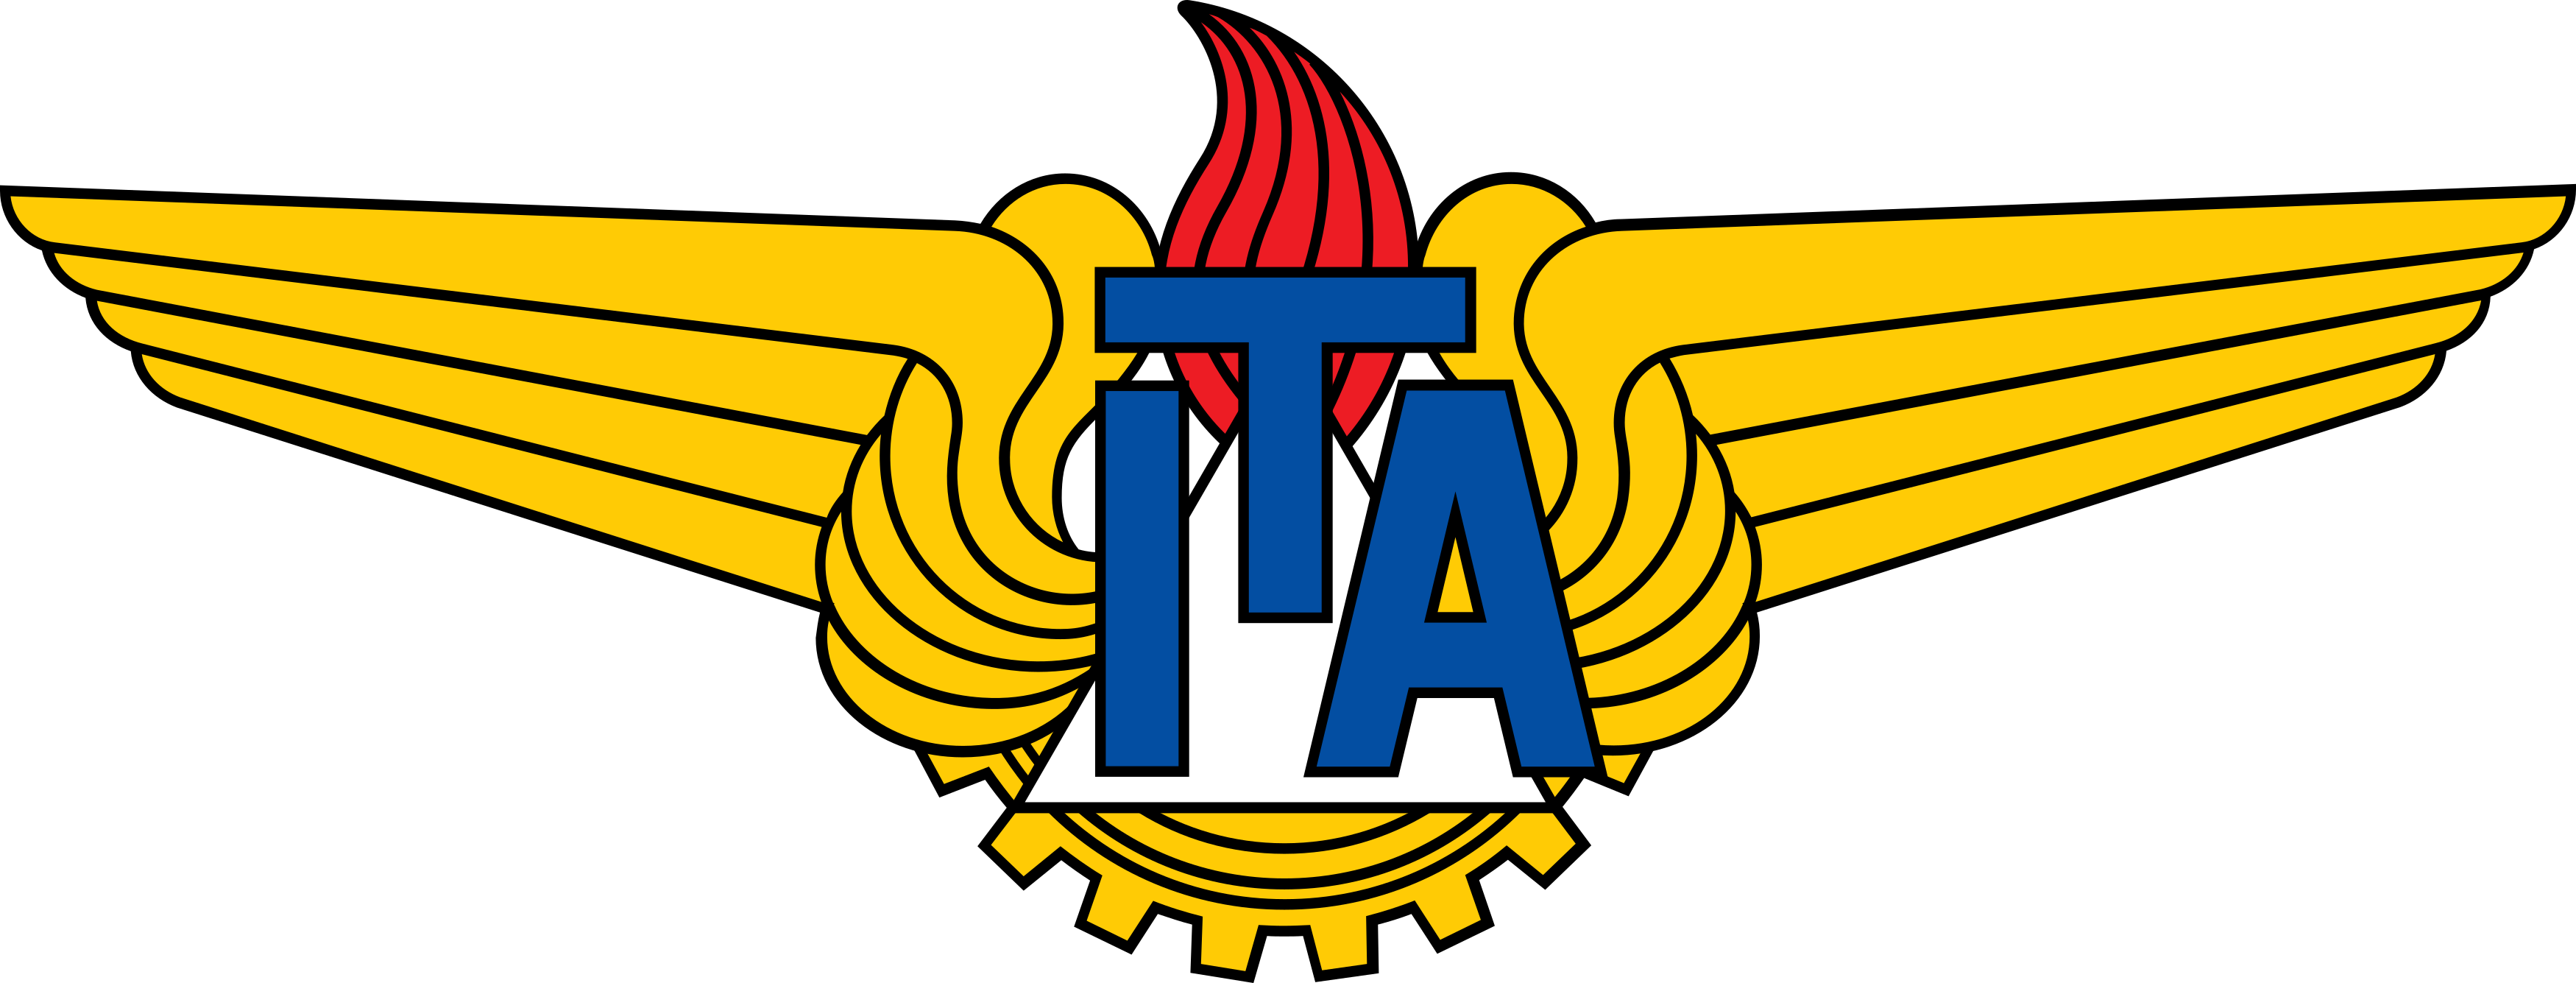
\includegraphics[width=9cm]{Images/ita-logo.png}
\end{center}
\end{figure}

\begin{huge}
\bf{\sc{Instituto Tecnológico de Aeronáutica}} \\
\vspace*{0.15in}
\end{huge}

\begin{Large}
\bf{\sc{Divisão de Engenharia Aeronáutica e Aeroespacial}}\\
\end{Large}

\begin{Large}
\vspace*{0.2in}
\textbf{Departamento de Eletrônica (IEE)} \\
\textbf{Projeto de ELE-27} \\

\vfill

\textbf{CubeSat}
\end{Large}

\vfill


\begin{large}
    \begin{FlushLeft}
        \textbf{Professor} \\
        Tertuliano Ribeiro Pinto \\
    \end{FlushLeft}
\end{large}

\begin{large}

\begin{FlushLeft}
    \textbf{Alunos} \\
    Ana Beatriz da Silva Machado\\
    Caio Jansen Accioly\\
    Lucas Ramalho Rocha\\
    Luísa Dallmann\\
    Mahmud Mohamad Hussein Ali Neto\\
    Mateus Silva Borges\\
    Natan Campistano de Mello\\
    Pedro Kuntz Puglia \\
\end{FlushLeft}

\end{large}
\vspace*{0.1in}
\Large{2023}
\end{center}
\end{titlepage}




\input{Tex/0.Sumário.tex}

\input{Tex/9.Referências.tex}

\end{document}

\mainmatter
% Os capitulos comecam aqui
\chapter{Introdução}
\section{Motivação e objetivos}



\chapter{Metodologia}

O trabalho foi iniciado com o projeto do motor a gás frio. A seguir, este motor foi validado experimentalmente em uma bancada de teste de empuxo. Com o sistema propulsivo pronto, projetou-se o sistema de \textit{jet vanes}. Por fim, este sistema foi aferido em uma balança de três componentes para medição do empuxo e força lateral gerada pelo sistema. 

\section{Projeto do motor}

O projeto do motor foi feito de maneira programática e iterativa, assegurando fácil reprodução dos resultados obtidos e automação do fluxo de dados. A linguagem de programação \textit{Julia} foi utilizada para o projeto. Nesta seção, serão apresentados os dados referentes à última versão do motor. Para um histórico do desenvolvimento do motor, consultar o apêndice AAAAAAAAAAA.  

A tabela~\ref{tab:requirements} mostra os requisitos propulsivos, codificados PRP-N, e geométricos, codificados GMT-N, levantados para o motor. Os requisitos PRP-1 e PRP-2 foram propostos com base nos sistemas de fornecimento de ar disponíveis e na escala desejada do motor. Já a temperatura do propelente, requisito PRP-2, é baseada na temperatura ambiente, e permite a utilização de \textit{jet vanes} feitas de materiais simples. Com base nestes requisitos, um sistema monopropelente a ar foi proposto. Os requisitos GMT-1 e GMT-2 foram especificados com base na necessidade de haver estagnação na câmara de empuxo (seção~\ref{sec:intro}) e na necessidade de fácil manipulação, manufatura e conexão. Já os requisitos GMT-3 e GMT-4 buscam propiciar um escoamento com alto paralelismo na região da tubeira, assim como facilitar a manufatura.

\begin{table}[]
    \centering\begin{tabular}{cccc} \toprule
        Código & Variável & Grandeza & Valor \\ \midrule
        PRP-1 & \(P_C\) & Pressão de câmara & \(500kPa\) \\
        PRP-2 & \(T\) & Empuxo & \(2N\) \\
        PRP-3 &\(T_{prop}\) & Temperatura do propelente & \(298,15K\) \\
        GMT-1 & \(r_{C,\text{min}}\) & Raio de câmara mínimo & \(15mm\) \\
        GMT-2 & \(L_C\) & Comprimento de câmara & \(30mm\) \\
        GMT-3 & \(\alpha_{\text{conv}}\) & Semi-ângulo do convergente & \(30^\circ \) \\
        GMT-4 & \(\alpha_{\text{div}}\) & Semi-ângulo do divergente & \(5^\circ \) \\ \bottomrule 
    \end{tabular}
    \caption{Requisitos propulsivos e geométricos para o motor.}
    \label{tab:requirements}
\end{table}

A partir destes requisitos, o software CEA NASA foi utilizado para calcular os parâmetros propulsivos (\(\varepsilon \), \(C^\ast \) e \(C_f\)) do sistema com pressão ambiente \(P_{amb} = 100kPa\). Com estes coeficientes, pode-se aplicar as relações~\ref{eq:exp_ratio} e~\ref{eq:C_F} descritas na seção~\ref{sec:intro} para calcular as áreas de saída \(A_e\), de garganta \(A_t\). A área de câmara, \(A_C\), foi calculada diretamente a partir do requisito GMT-1. Foi introduzida uma seção cilíndrica na garganta do motor, com área de seção transversal \(A_t\), para garantir a manufatura precisa dessa dimensão.

Os três coeficientes propulsivos calculados também foram utilizados para estimar o fluxo mássico de propelente \(\dot{m}\), e este, para estimar a velocidade do propelente na mangueira de alimentação, \(v_{\text{prop}}\). Estes parâmetros são relevantes para a verificação da perda de carga no sistema de alimentação, bem como para a escolha da fonte de ar. Como o propelente é pouco energético, altas vazões são necessárias mesmo para empuxos pequenos, de modo que conhecer a capacidade exigida da fonte foi fundamental. A partir de \(\dot{m}\), cujo cálculo foi descrito anteriormente, e assumindo que a  um diâmetro de tubo \(d\), massa molar do ar \(MM_{ar}\) e constante dos gases \(R\):
\begin{equation}
    v_{\text{prop}} = \frac{\dot{m} R T_{\text{prop}}}{\pi \left(\frac{d}{2}\right)^2 P_C MM_{ar}}
\end{equation}

Com as áreas das seções transversais do motor calculadas, e em posse da especificação da geometria interna do motor, gerou-se o CAD do motor para impressão 3D. Em \textit{Julia}, utilizou-se a package \textit{ConstructiveGeometry}\footnote[1]{https://github.com/plut/ConstructiveGeometry.jl} para gerar a geometria tridimensional a partir do dados de geometria calculados. Ao produzir o CAD diretamente a partir do código de projeto, foi possível eliminar etapas manuais que podem introduzir erros e atrasos ao projeto. A impressão 3D foi escolhida como método de manufatura devido à baixa temperatura de operação do motor, e à sua geometria complexa, assim como pela velocidade de prototipagem propiciada por esta tecnologia. O material de impressão usado foi ABS.\@

\section{Validação do projeto do motor}

O motor projetado e impresso em 3D foi montado em uma bancada de testes e instrumentado com os sensores da tabela ref. Os sensores, bem como uma válvula de gás comandada eletronicamente, foram ligados a um Arduino Mega para leitura e controle do conjunto de testes. 

%https://www.arduino.cc/reference/en/libraries/max6675/

\begin{table}[htbp]
    \centering\begin{tabular}{p{0.15\textwidth}p{0.5\textwidth}p{0.2\textwidth}} \toprule
        Sensor & Montagem & Biblioteca usada \\ \midrule
        Termopar & Inserido lateralmente na câmara de empuxo, selado com cola de ABS & MAX6675 \\
        Célula de carga & Apoio para o motor, sentido de medida paralelo ao empuxo & HX711 \\
        Transdutor de pressão & Acoplado à câmara de empuxo em furo lateral; ver CAD na seção RESULTADOS & Leitura analógica simples \\ \bottomrule
    \end{tabular}
    \caption{Descrição dos periféricos usados nos testes de validação do motor desenvolvido.}
    \label{tab:validation_peripherals}
\end{table}

Para o controle da bancada foi desenvolvida uma \textit{command line interface} simples para permitir testes interativos. Assim, as funções de tara, calibração, abertura e fechamento de válvula e leitura de sensores podiam ser comandadas a partir de uma interface textual interativa que facilitou a iteração do teste.

\section{Projeto do sistema de \textit{jet vanes}}

Devido à disponibilidade de materiais, foi utilizada uma lâmina de aço de 0,7mm de espessura como \textit{jet vane}. Com este sistema, desejou-se a capacidade de posicionar a lâmina defletora com resolução de \(1^\circ \), com alcance de deflexão de \(\pm 20^\circ \). Também foi necessário projetar um suporte para o motor que permitisse a conexão da mangueira de alimentação de gás. Por fim, este sistema deveria ter um encaixe circular de \(12mm\) para um eixo de acoplamento com a balança de três componentes.

\section{Caracterização do sistema em balança de três componentes}

\chapter{Resultados}

\section{Projeto do motor}

Da metodologia e dos requisitos expostos na seção~\ref{sec:motor_project}, foi gerada a geometria do motor para impressão 3D. A figura~\ref{fig:internal_profile} mostra a seção longitudinal projetada para o motor. Destaca-se o grande volume da câmara em comparação com a tubeira, devido à necessidade de haver estagnação de um escoamento intenso (ver vazão mássica adiante).

\begin{figure}[htbp]
    \centering
    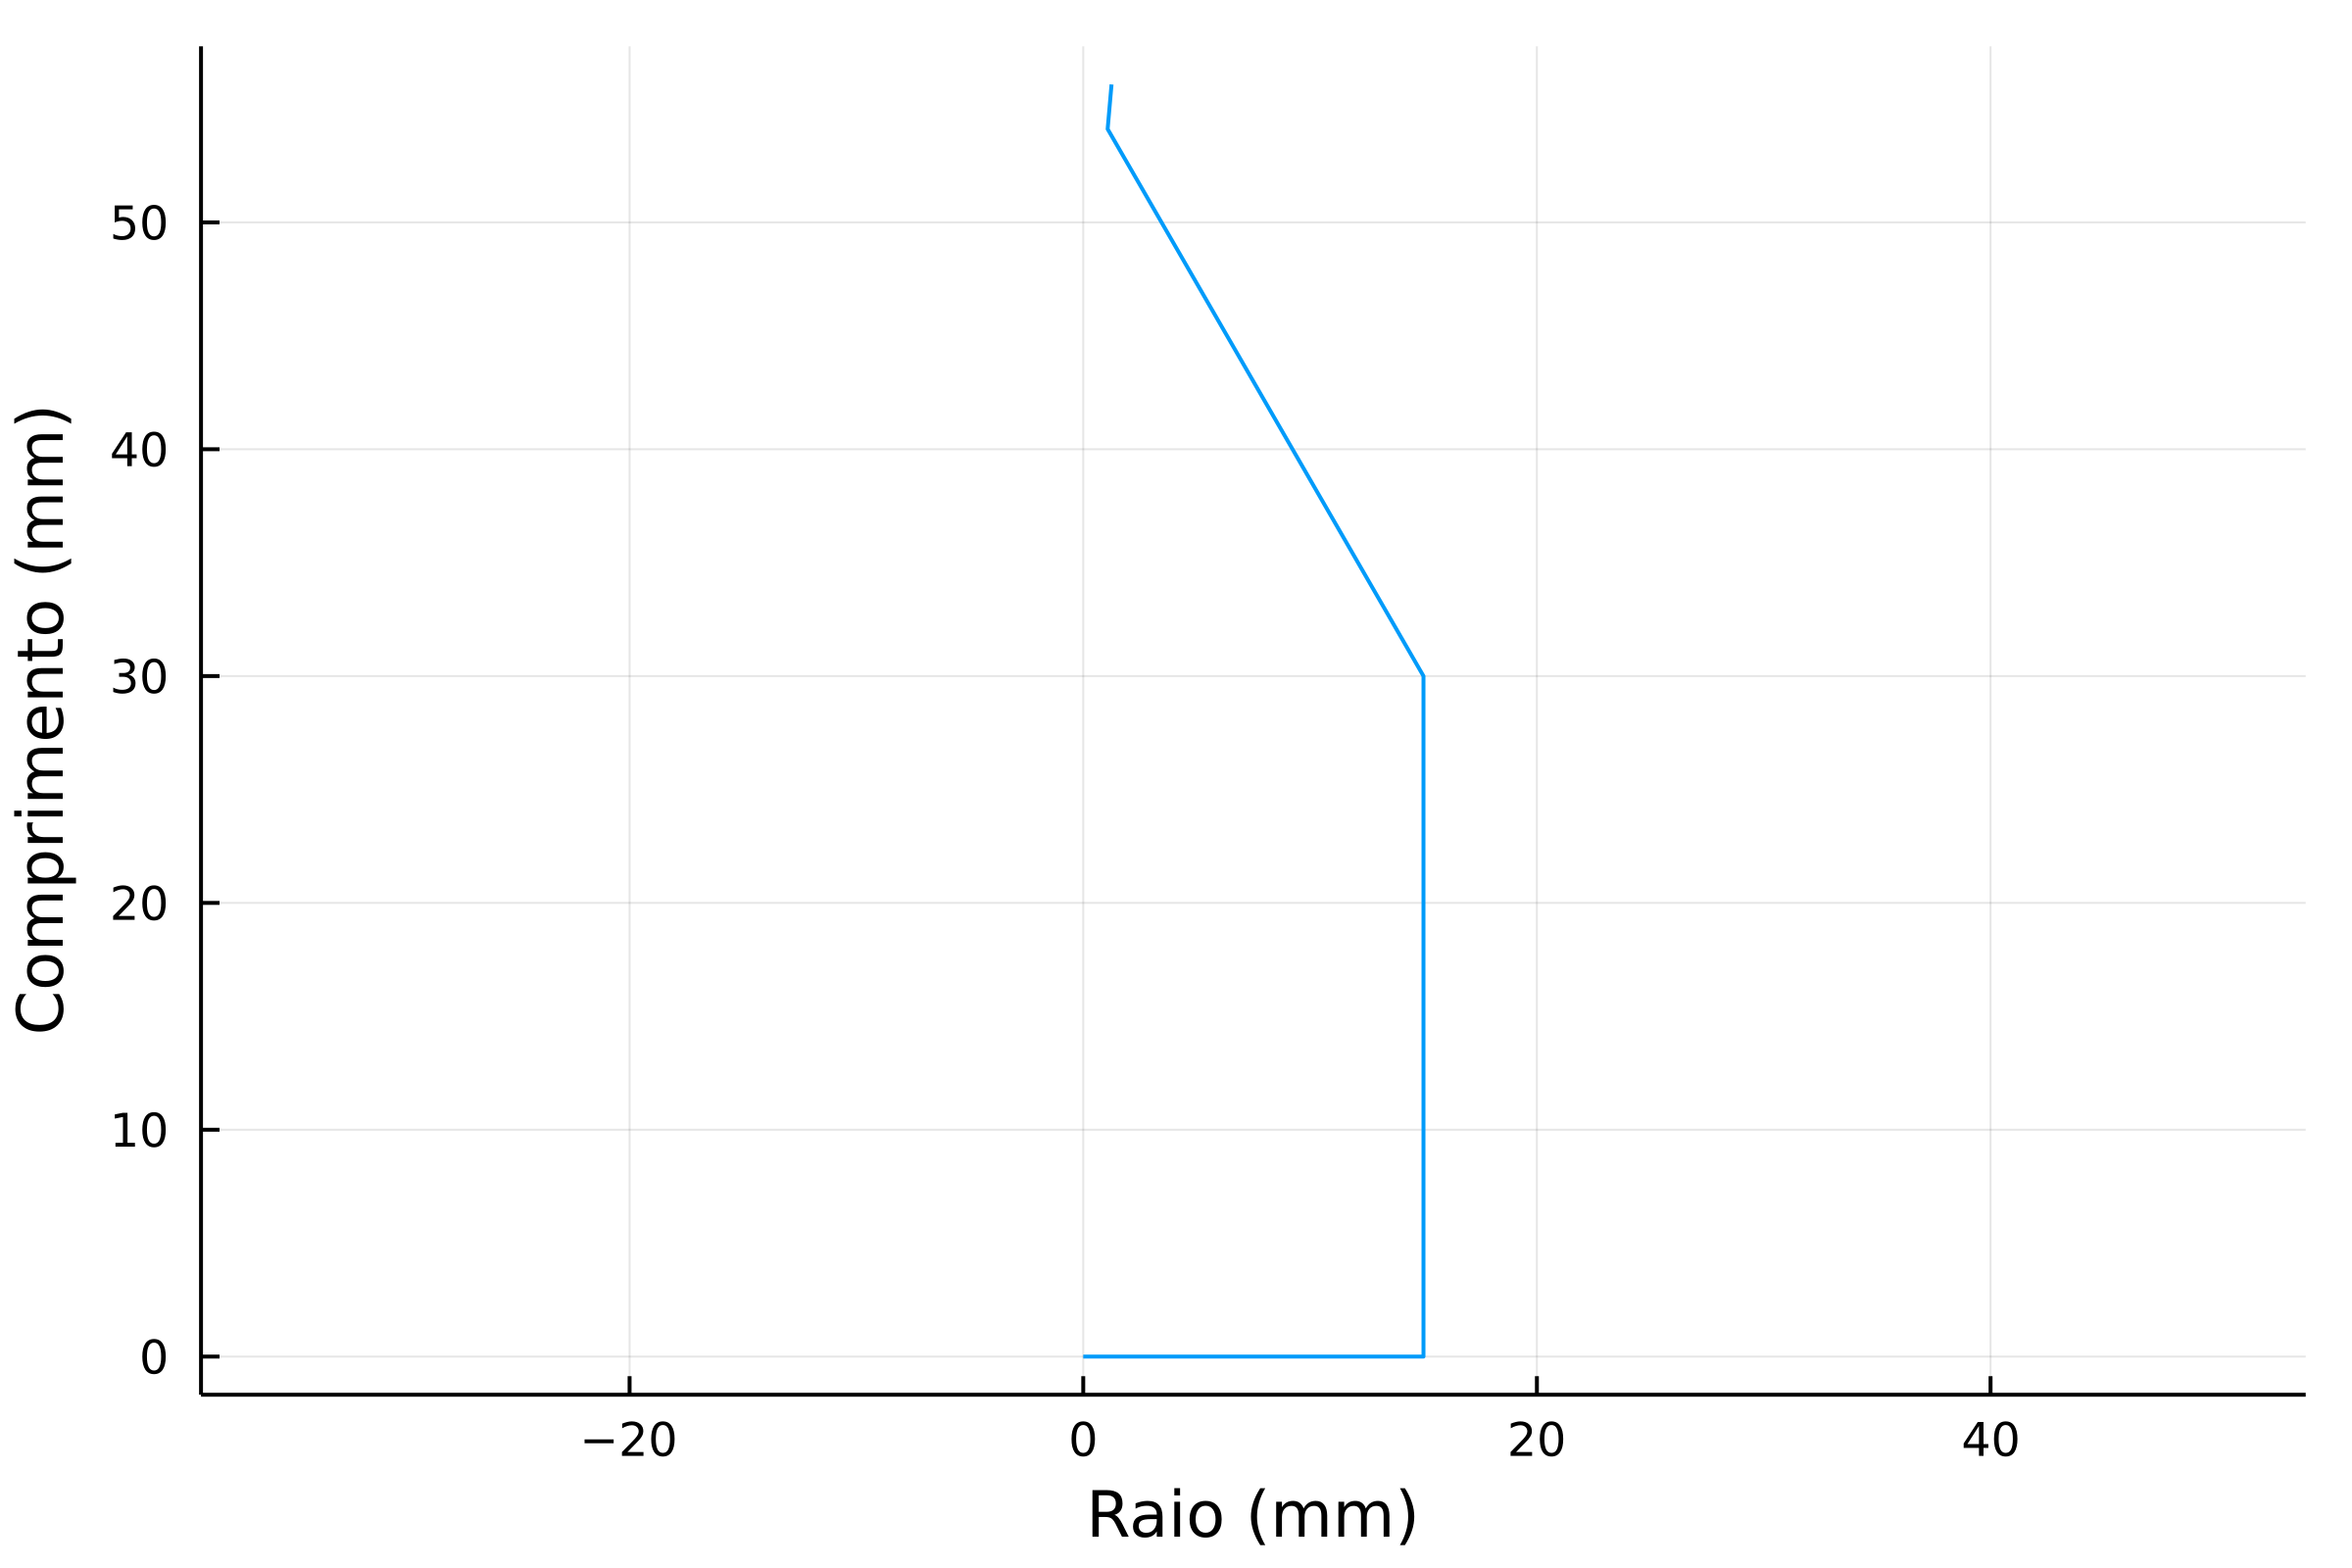
\includegraphics[width=\textwidth]{img/internal_profile.png}
    \caption{Perfil interno do motor projetado.}\label{fig:internal_profile}
\end{figure}

Os parâmetros propulsivos calculados para o motor foram:
\begin{itemize}
    \item \( \varepsilon = 1,35 \)
    \item \(C^* = 427,2\;\mathrm{m}\,\mathrm{s}^{-1}\)
    \item \(C_{F} = 1,10\)
\end{itemize}

Observa-se que o pequeno valor de razão de expansão é refletido na pequena tubeira exibida na figura~\ref{fig:internal_profile}. Foi obtido também um impulso específico de \(I_{sp} = 47,9s\) e um fluxo mássico de \(\dot{m} = 4,257\;\mathrm{g}\,\mathrm{s}^{-1}\). Devido à baixa energia do propelente, a velocidade característica do motor é bastante baixa, de modo que é necessário um fluxo mássico bastante elevado para a produção do empuxo requisitado. Isso é refletido no valor de impulso específico baixo. Ressalta-se também que o motor foi ajustado para operar à pressão ambiente, fator que limitou a razão de expansão e, portanto, o coeficiente de empuxo. 

O perfil da figura~\ref{fig:internal_profile} foi revolucionado para se obter uma geometria tridimensional cilíndrica, com superfícies planas externas adicionadas para facilitar a manufatura e a conexão com mangueiras de gás. Na figura~\ref{fig:3d_geom}, à esquerda, observa-se a geometria STL gerada em código para o motor. Foi adicionado um furo lateral para conexão com uma mangueira de alimentação, bem como quatro superfícies planas laterais para facilitar o manuseio e o apoio em morsas e outros equipamentos. À direita, observa-se o motor real construído. Destacam-se aqui as ranhuras da rosca para conexão da mangueira de gás.

\begin{figure}[htbp]
    \centering
    \begin{subfigure}{0.49\textwidth}
        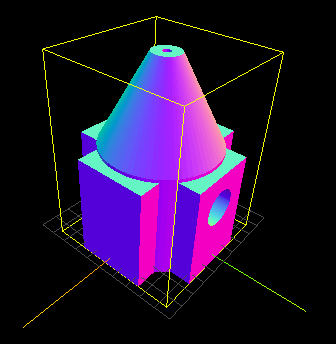
\includegraphics[width=\textwidth]{img/motor_stl.png}
        \caption{Geometria STL gerada para o motor.}
    \end{subfigure}
    \begin{subfigure}{0.49\textwidth}
        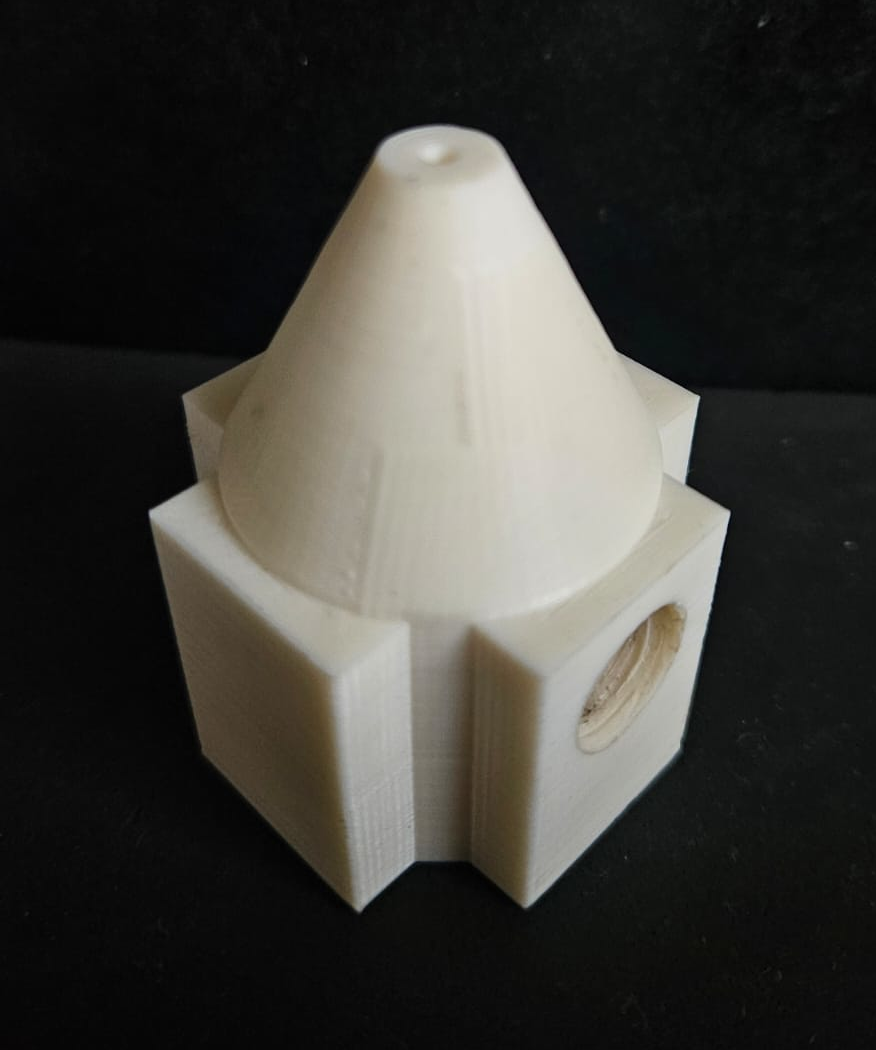
\includegraphics[width=\textwidth]{img/motor_real.png}
        \caption{Motor impresso em 3D.}
    \end{subfigure}
    \caption{Geometria tridimensional do motor projetado.}\label{fig:3d_geom}
\end{figure}

\section{Validação do projeto do motor}\label{sec:result_validation}

A bancada de testes descrita na seção~\ref{sec:method_validation} gerou dados de empuxo para o motor e pressão estática e temperatura de câmara. A temperatura manteve-se bastante constante, próxima do valor especificado no requisito PRP-3, de modo que ela será tratada como constante e idêntica a este valor. O gráfico~\ref{fig:thrust_versus_p1} exibe as medidas de empuxo feitas em função da pressão de câmara medida.

\begin{figure}[htbp]
    \centering
    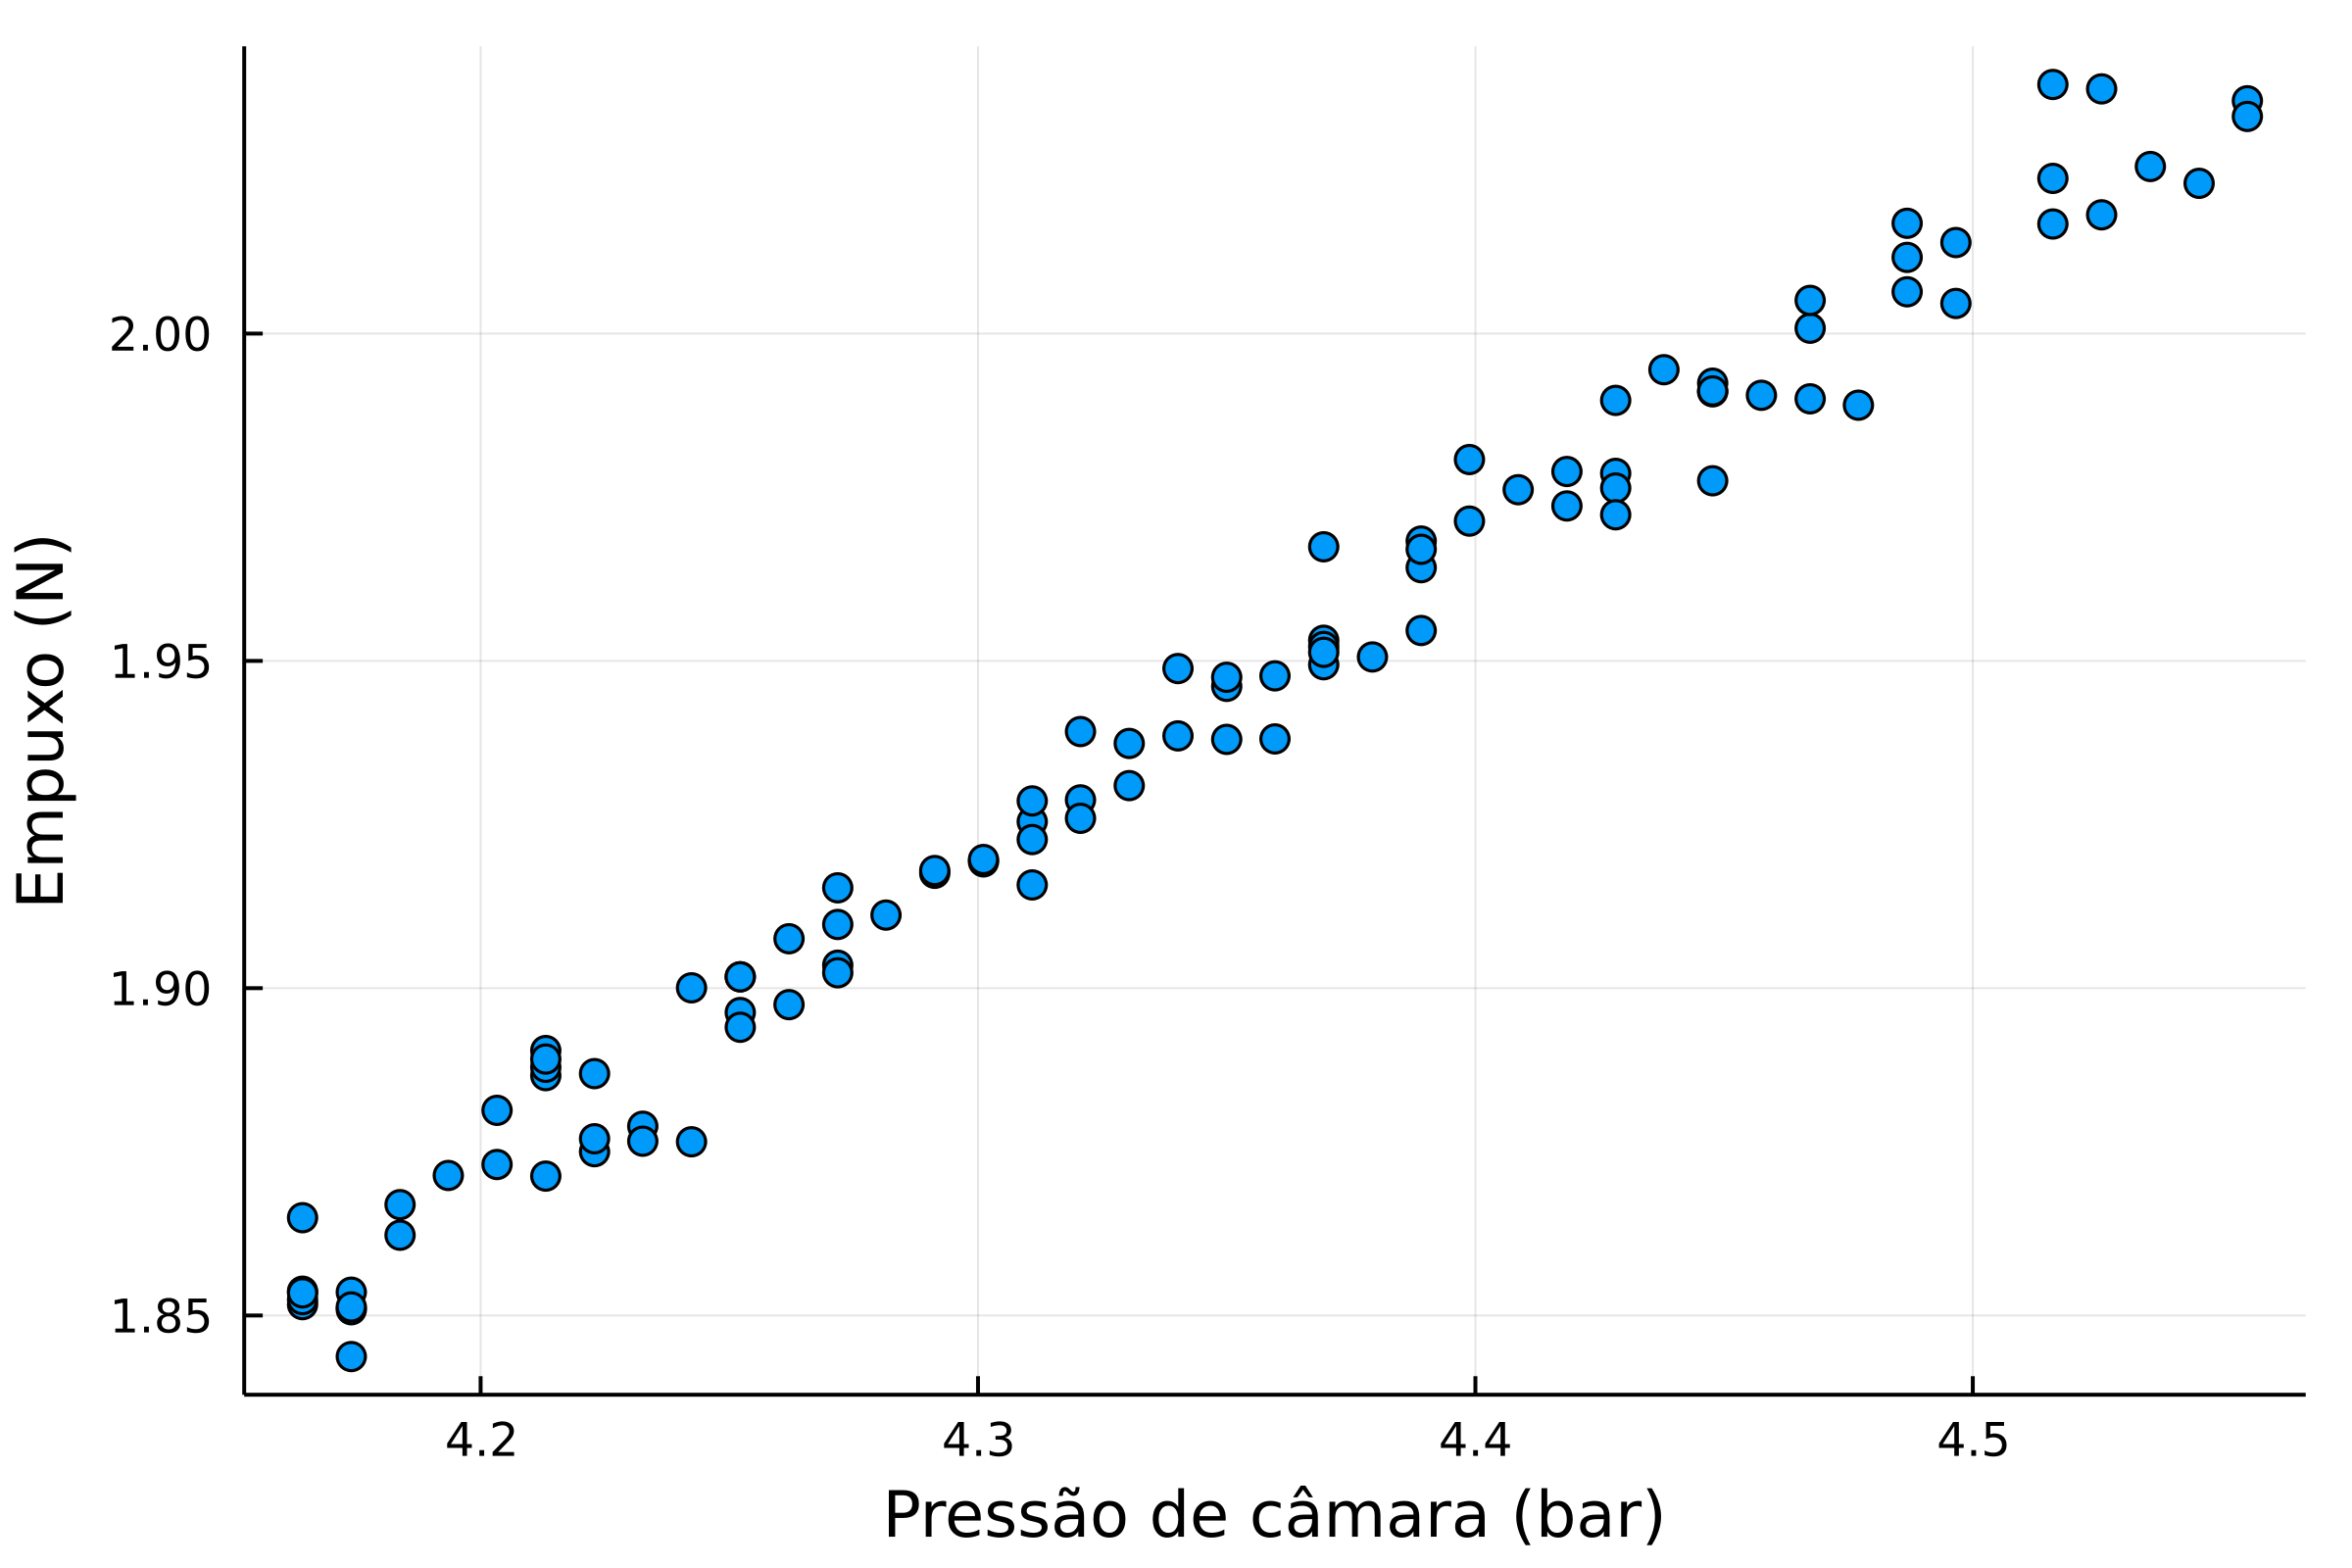
\includegraphics[width=\textwidth]{img/thrust_vs_chamber_pressure.png}
    \caption{Empuxo em função de pressão de câmara estática.}\label{fig:thrust_versus_p1}
\end{figure}

A variação de pressão de câmara observada neste ensaio deve-se ao grande fluxo mássico exigido pelo motor, que causou esvaziamento significativo do compressor de ar utilizado durante o teste. Também destaca-se que a pressão medida na câmara, entre \(4,2bar\) e \(4,6bar\), foi inferior à pressão regulada em válvula, de exatamente \(5bar\). No entanto, o fato do motor real atingir os \(2N\) de empuxo exigidos com pressão próxima de \(4,5bar\) permitiu que a pesquisa continuasse levando-se em consideração as diferenças entre o motor real e o motor projetado.

Parâmetros propulsivos reais podem ser obtidos dos dados apresentados na figura~\ref{fig:thrust_versus_p1} através das equações~\ref{eq:C_F} e~\ref{eq:cstar}. Seus valores médios, com incerteza \(1\sigma \) são apresentados a seguir. A \(2N\) de empuxo, obteve-se impulso específico de \(46,6s\).
\begin{align}
    C_F &= 1,228 \pm 0,005 \\
    C^* &= (368,8 \pm 2,4)\;\mathrm{m}\,\mathrm{s}^{-1}
\end{align}

\section{Projeto do sistema de \textit{jet vanes}}\label{sec:result_jet_vanes}

Foi projetada uma montagem de suporte para o motor foguete, para o servomotor e para o mecanismo da lâmina defletora. A figura~\ref{fig:jet_vanes_render1} mostra este mecanismo em posição neutra. À esquerda tem-se o servomotor, acoplado a um braço extensor, que se conecta mecanicamente com uma peça de suporte da lâmina defletora. A lâmina é suportada em ambas as extremidades para garantir rigidez estrutural à peça. O suporte da lâmina defletora pode girar ao redor de seu centro, com um mancal visível no canto superior direito da figura. Logo abaixo deste suporte, é possível observar o furo de conexão com o eixo da balança de três componentes, descrita anteriormente. A peça alta imediatamente à direita do servomotor é o suporte para o motor foguete, cuja tubeira fica próxima à lâmina defletora. O recesso semicircular no topo desta peça permite a conexão do motor com uma mangueira de alimentação de gás frio.

\begin{figure}[htbp]
    \centering
    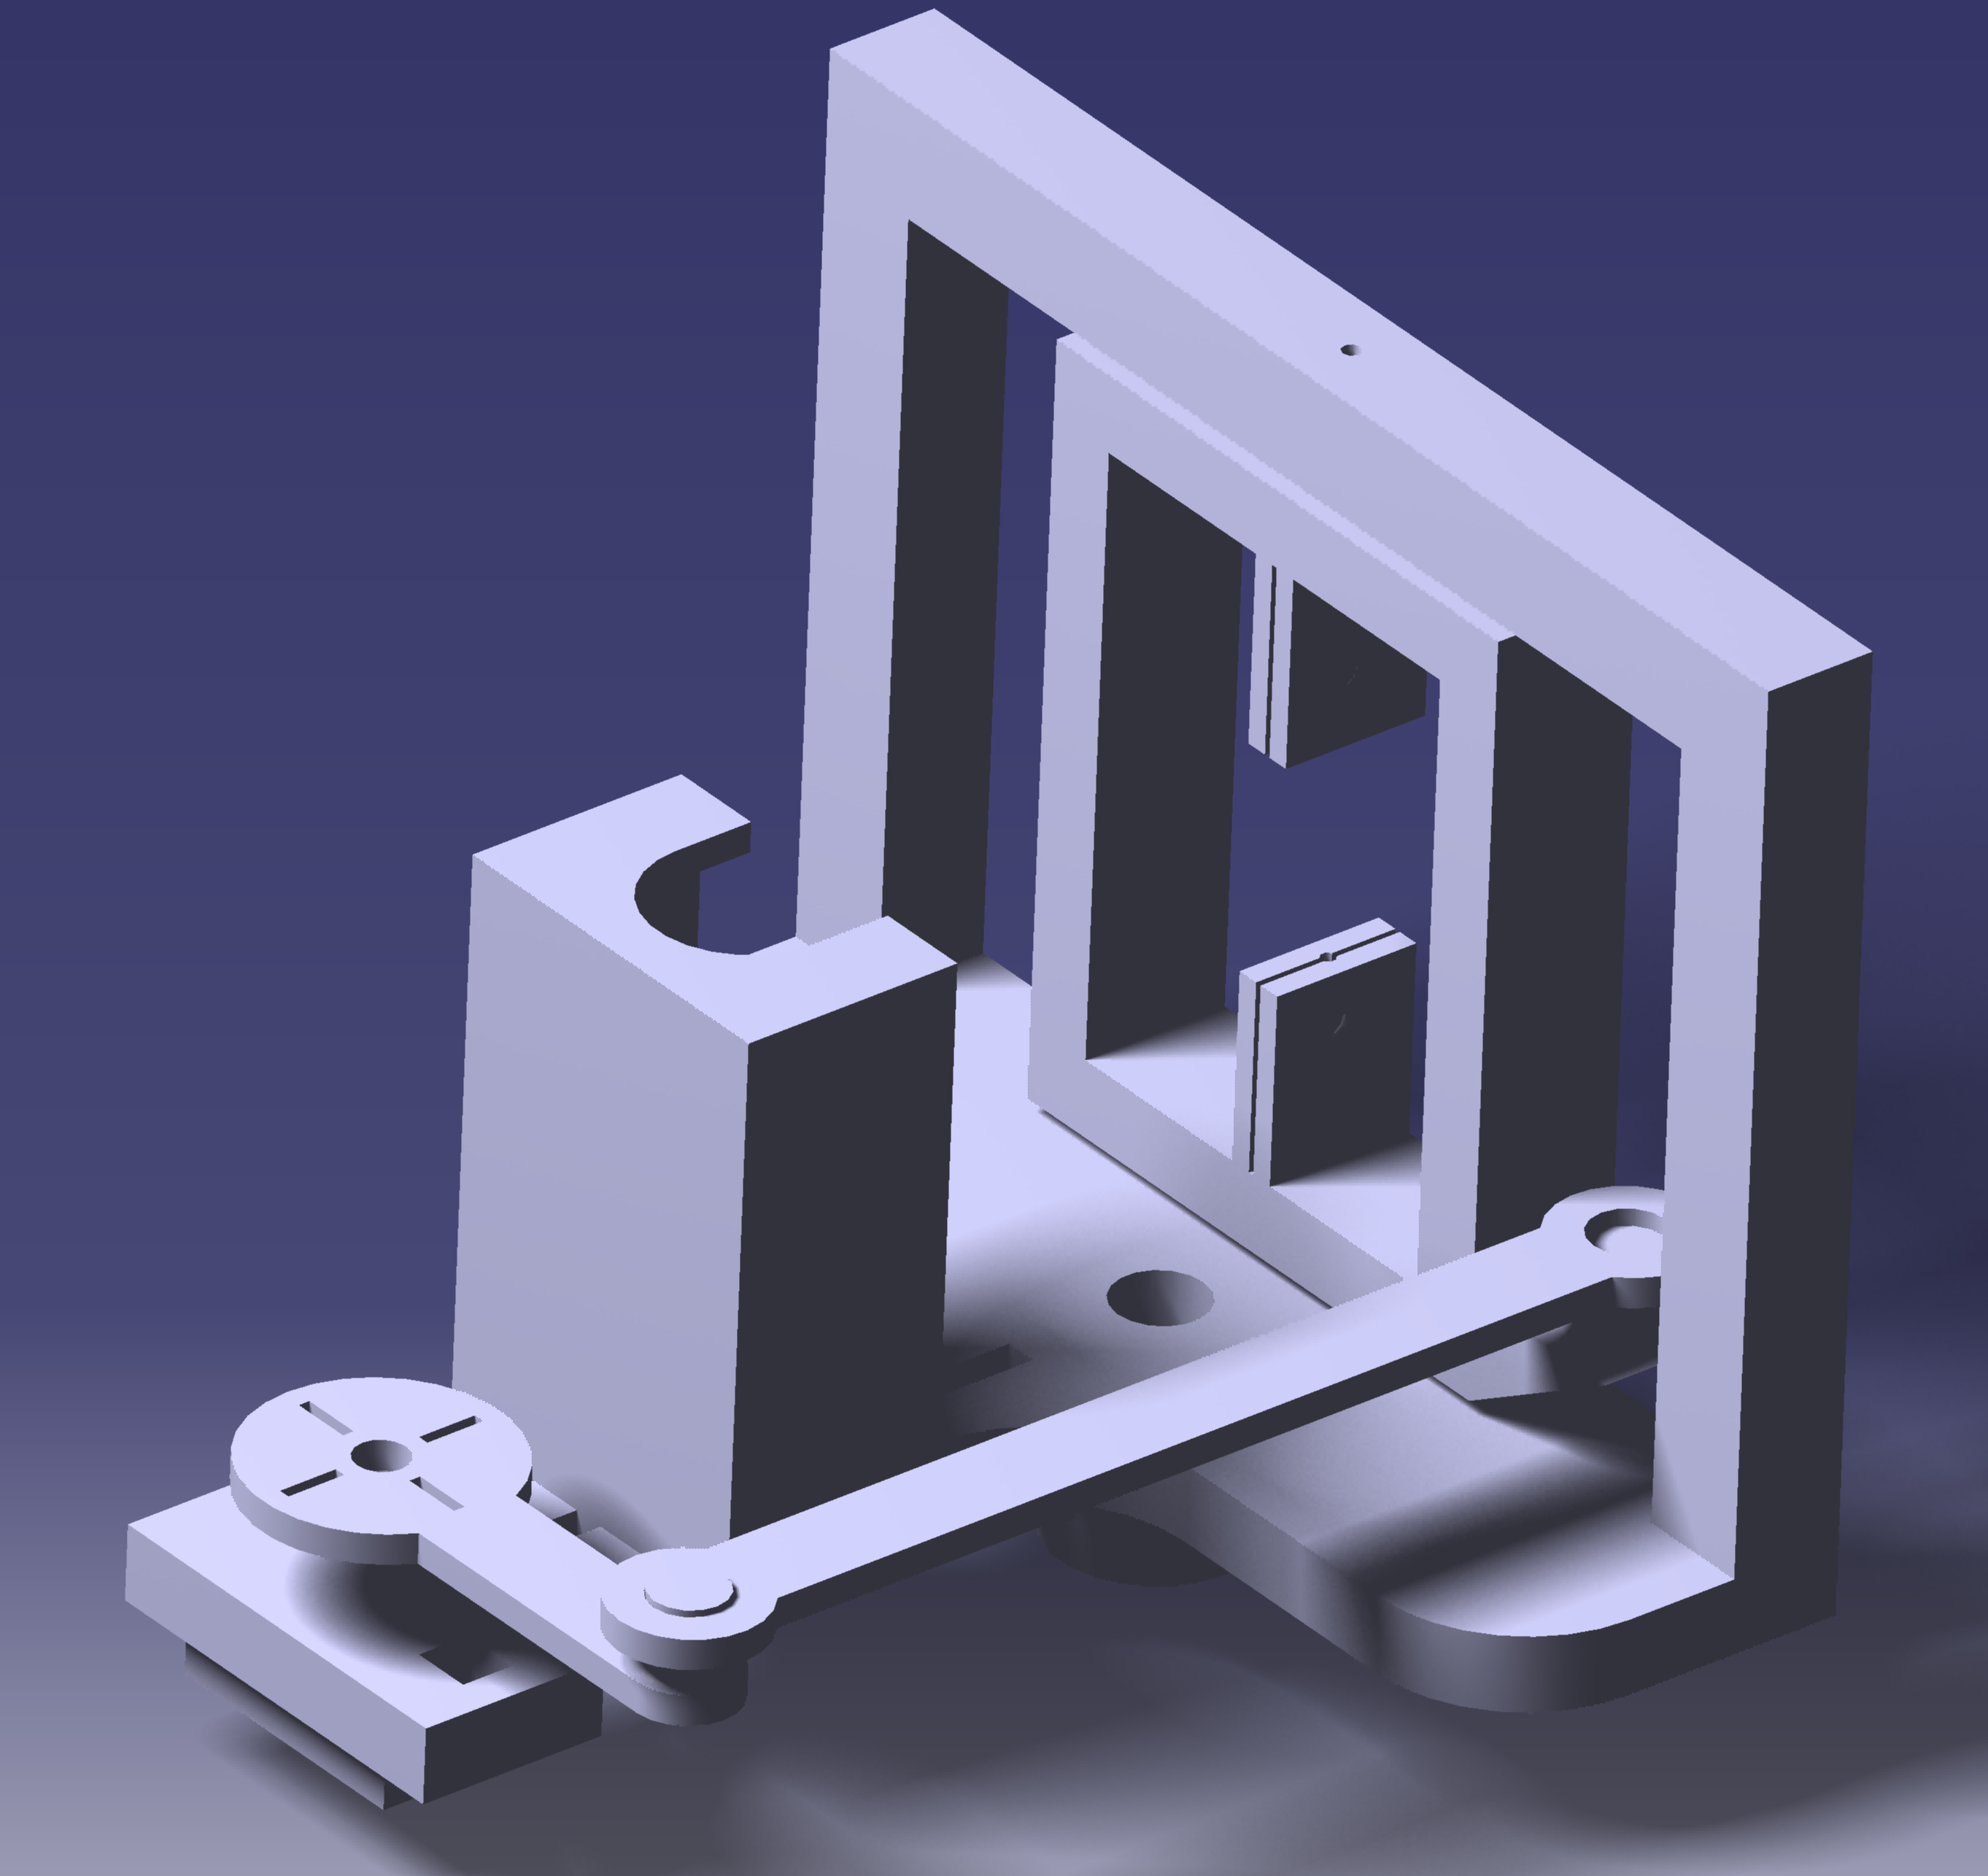
\includegraphics[width=\textwidth]{img/tvc_assembly_render1.png}
    \caption{Montagem do sistema de \textit{jet vanes} renderizada no CATIA.}\label{fig:jet_vanes_render1}
\end{figure}

A figura~\ref{fig:jet_vanes_render2} demonstra o funcionamento do mecanismo projetado em CAD\@. Foram impostos à montagem em CAD \textit{constraints} mecânicos que simulam o comportamento pretendido do sistema, de modo que os graus de liberdade das peças estejam adequadamente representados. O ângulo de rotação do servomotor é transmitido ao suporte da lâmina defletora através de uma haste longitudinal. Por projeto, os raios dos encaixes desta haste no servomotor e no suporte da lâmina defletora são iguais, de modo que os ângulos de deflexão são idênticos. O extensor do servomotor foi calibrado para que apresentasse posição perpendicular ao eixo longitudinal da montagem quando o servomotor recebesse um comando de \(90\mathrm{^\circ}\). O comprimento da haste foi estabelecido de modo que o suporte da lâmina defletora ficasse paralelo ao servomotor.

\begin{figure}[htbp]
    \centering
    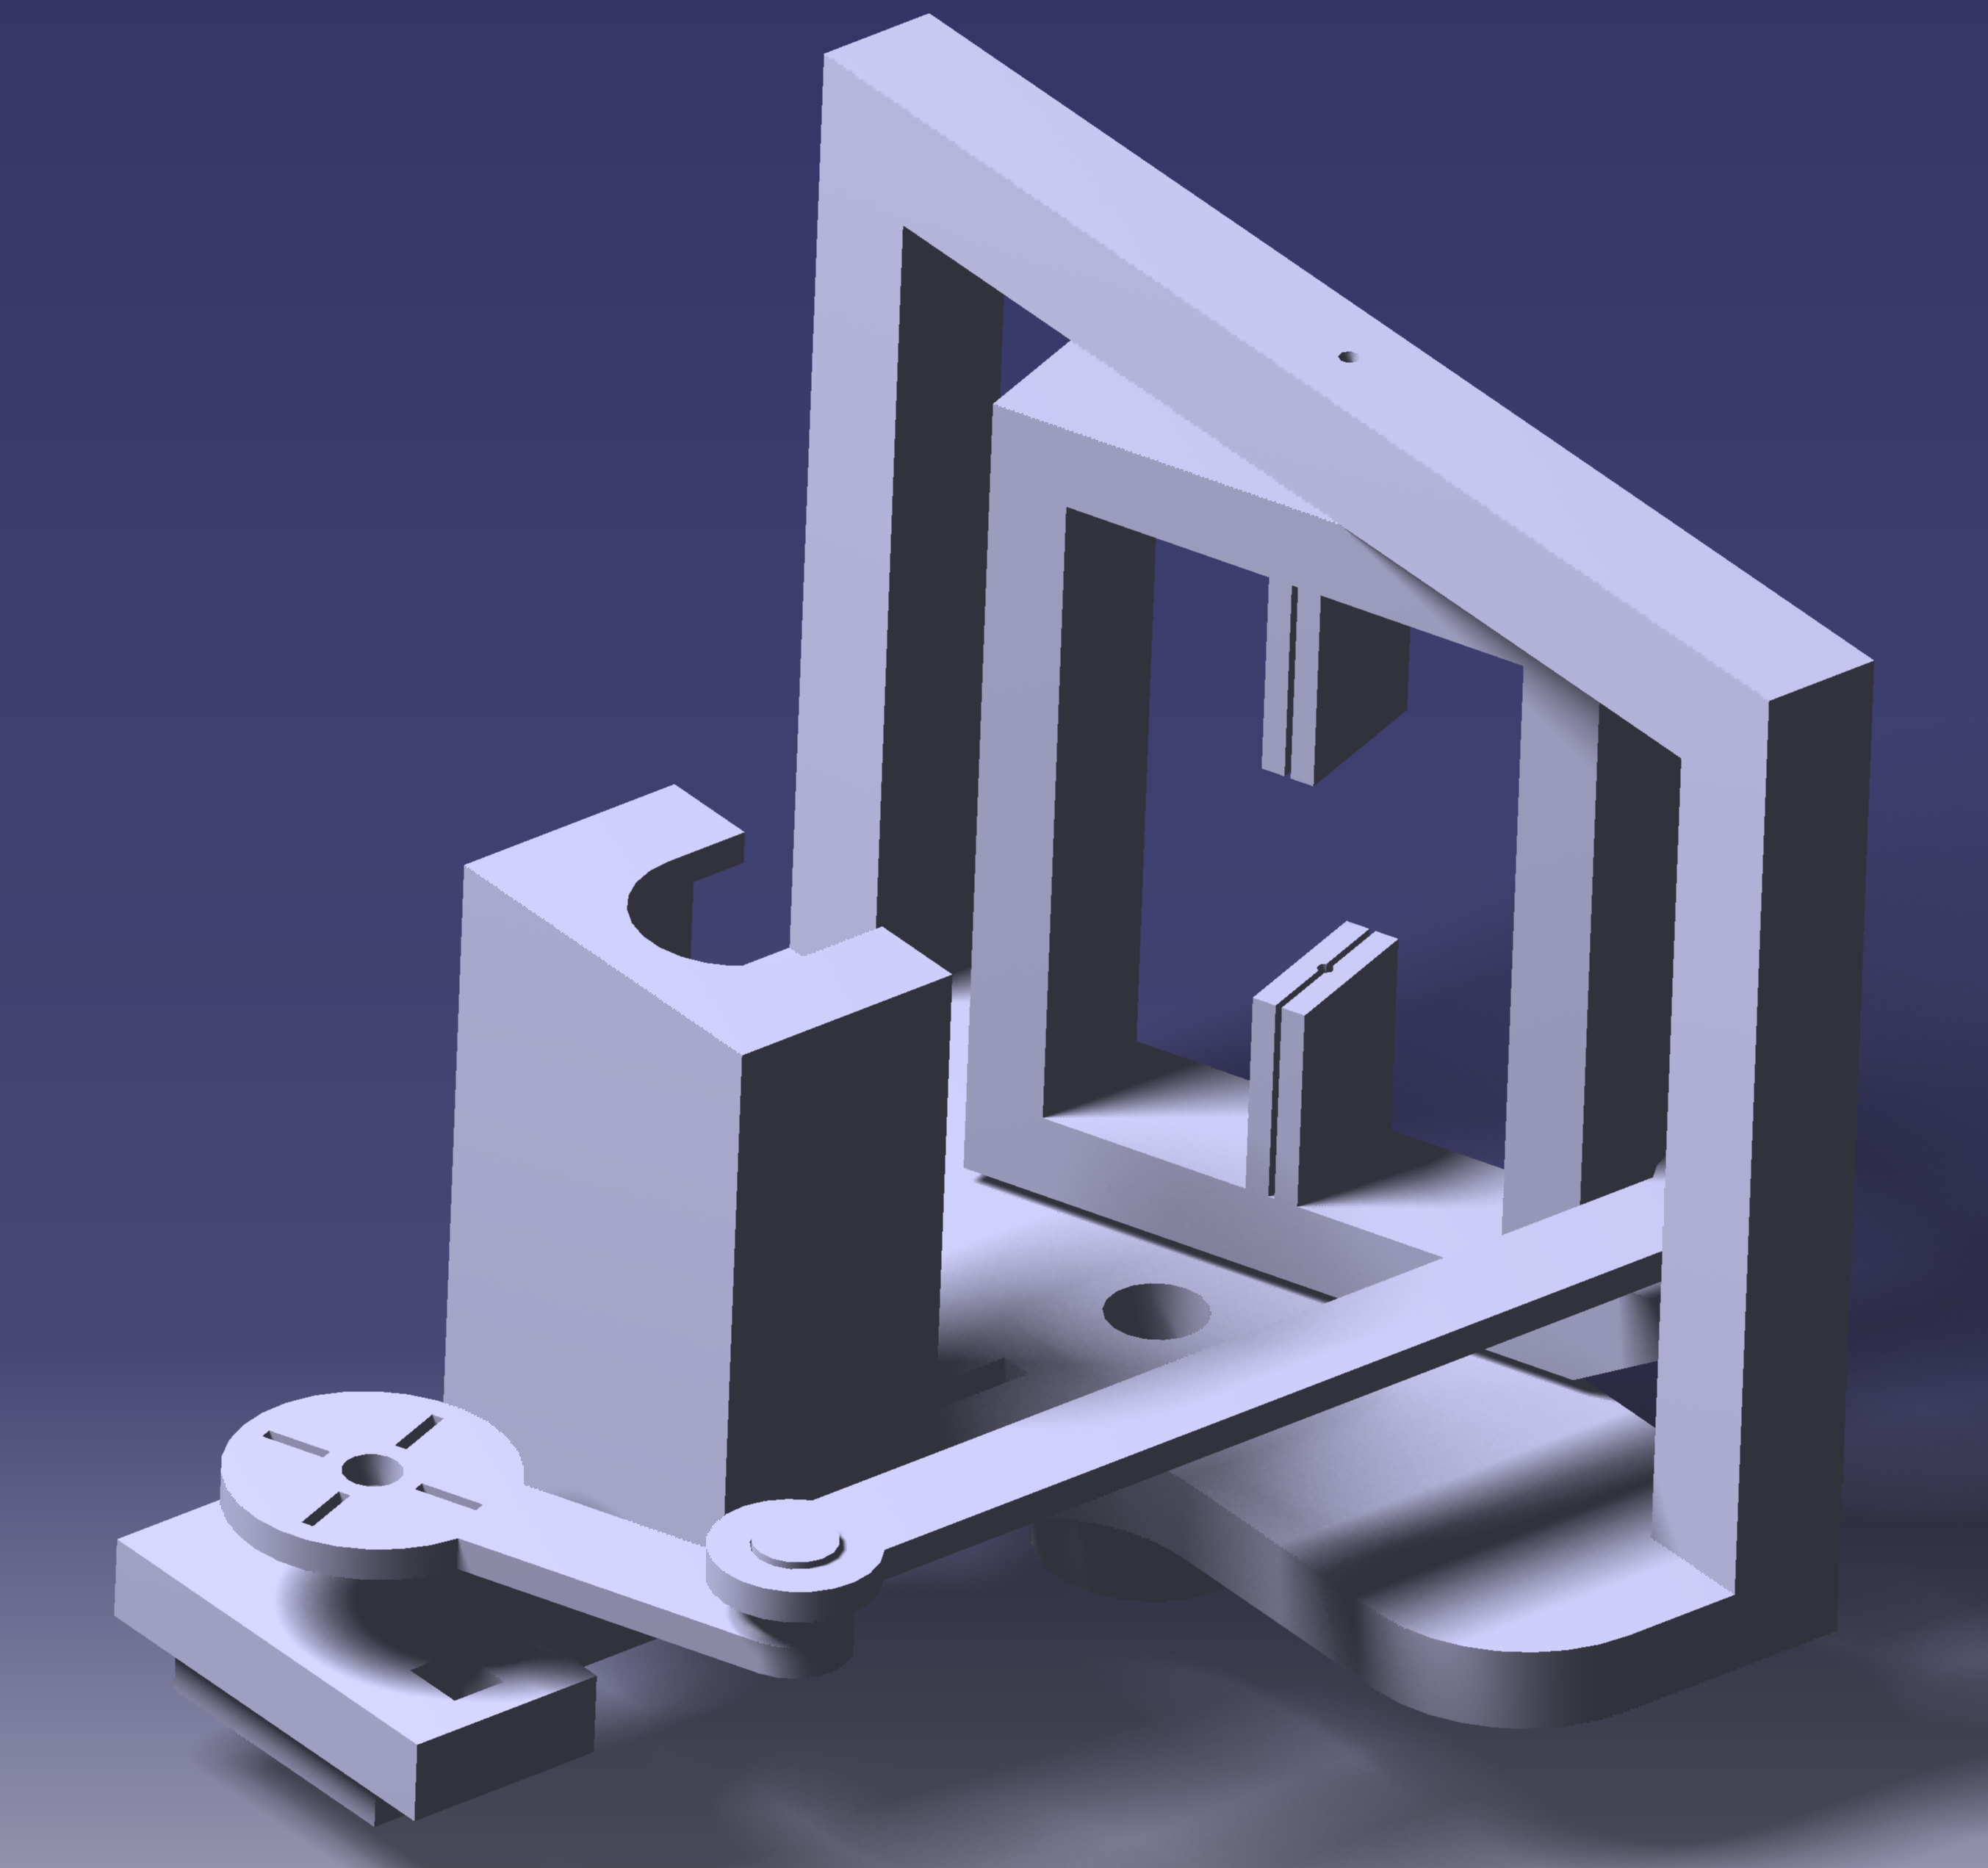
\includegraphics[width=\textwidth]{img/tvc_assembly_render2.png}
    \caption{Sistema de \textit{jet vanes} defletido de \(20\mathrm{^\circ}\).}\label{fig:jet_vanes_render2}
\end{figure}

As peças projetadas foram então impressas em 3D e montadas. A figura~\ref{fig:jet_vanes_assembly_side} mostra uma vista lateral do mecanismo. Destaca-se aqui o motor foguete montado em seu suporte, com um conector de mangueira de gás frio acoplado. Destaca-se também o eixo de metal à direita, usado para o encaixe na balança de três componentes utilizada.

\begin{figure}[htbp]
    \centering
    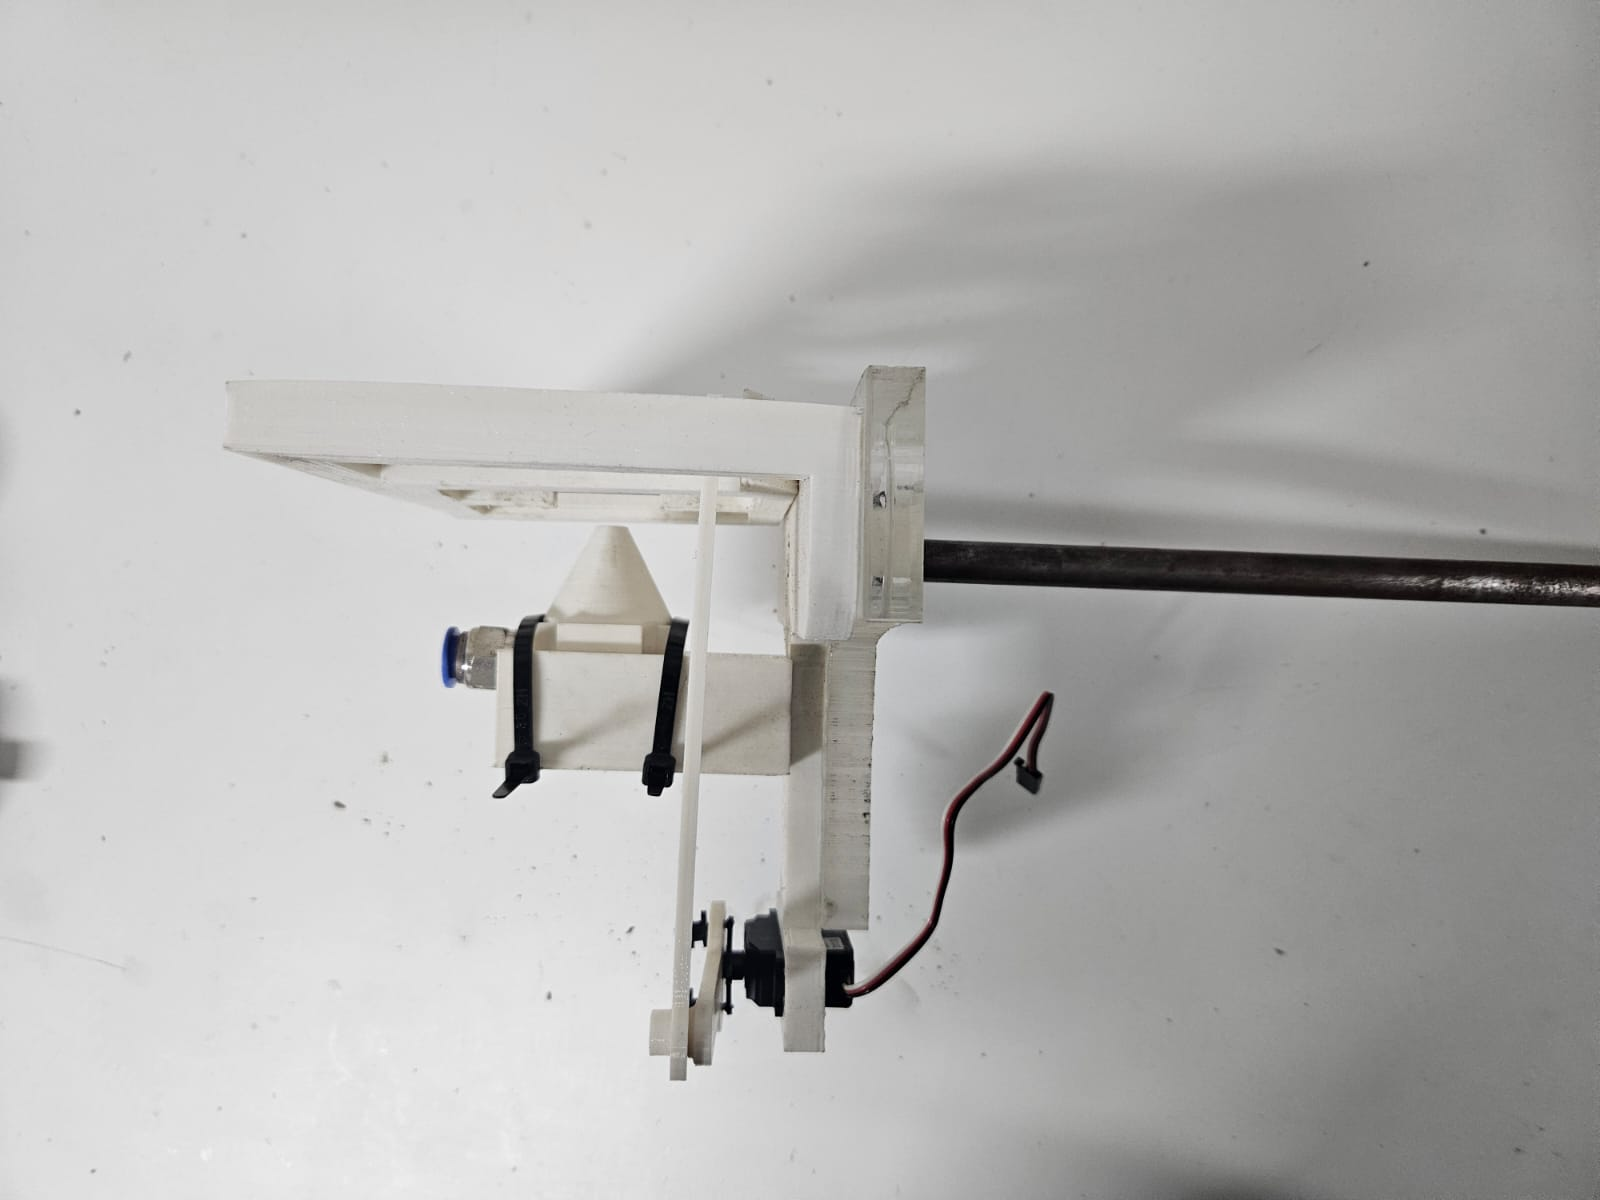
\includegraphics[width=\textwidth]{img/tvc_assembly_left.jpeg}
    \caption{Vista lateral do sistema de \textit{jet vanes} impresso e montado.}\label{fig:jet_vanes_assembly_side}
\end{figure}


\section{Caracterização do sistema em balança de três componentes}\label{sec:result_characterization}

As curvas de calibração dos componentes da balança estão exibidas na figura~\ref{fig:calibration_curves}. A curva vermelha tracejada indica a função identidade, ou seja, a igualdade exata entre a força calibrada e a força aplicada durante a calibração. Os pontos azuis indicam a força calculada através da calibração feita, usando a saída da balança para um dado carregamento. Nesta seção, todas as barras de erro referem-se ao erro quadrático médio obtido ao longo de \(1s\) de medida com amostragem de \(1000\mathrm{Hz}\). A calibração foi feita com dados de carregamento e descarregamento da balança para que a histerese dos componentes fosse observável, como na figura~\ref{fig:calibration_FF}. Destaca-se também que devido ao posicionamento do sistema, a força horizontal esperada era simétrica ao redor de zero, de modo que a componente \(F_D\) foi calibrada simetricamente ao redor de zero. Observa-se também que o zero das curvas apresentadas é referenciado em relação ao pré-carregamento aplicado, conforme explicado na seção~\ref{sec:method_3axis_measurement}.

\begin{figure}[htbp]
    \centering
    \begin{subfigure}{\textwidth}\centering
        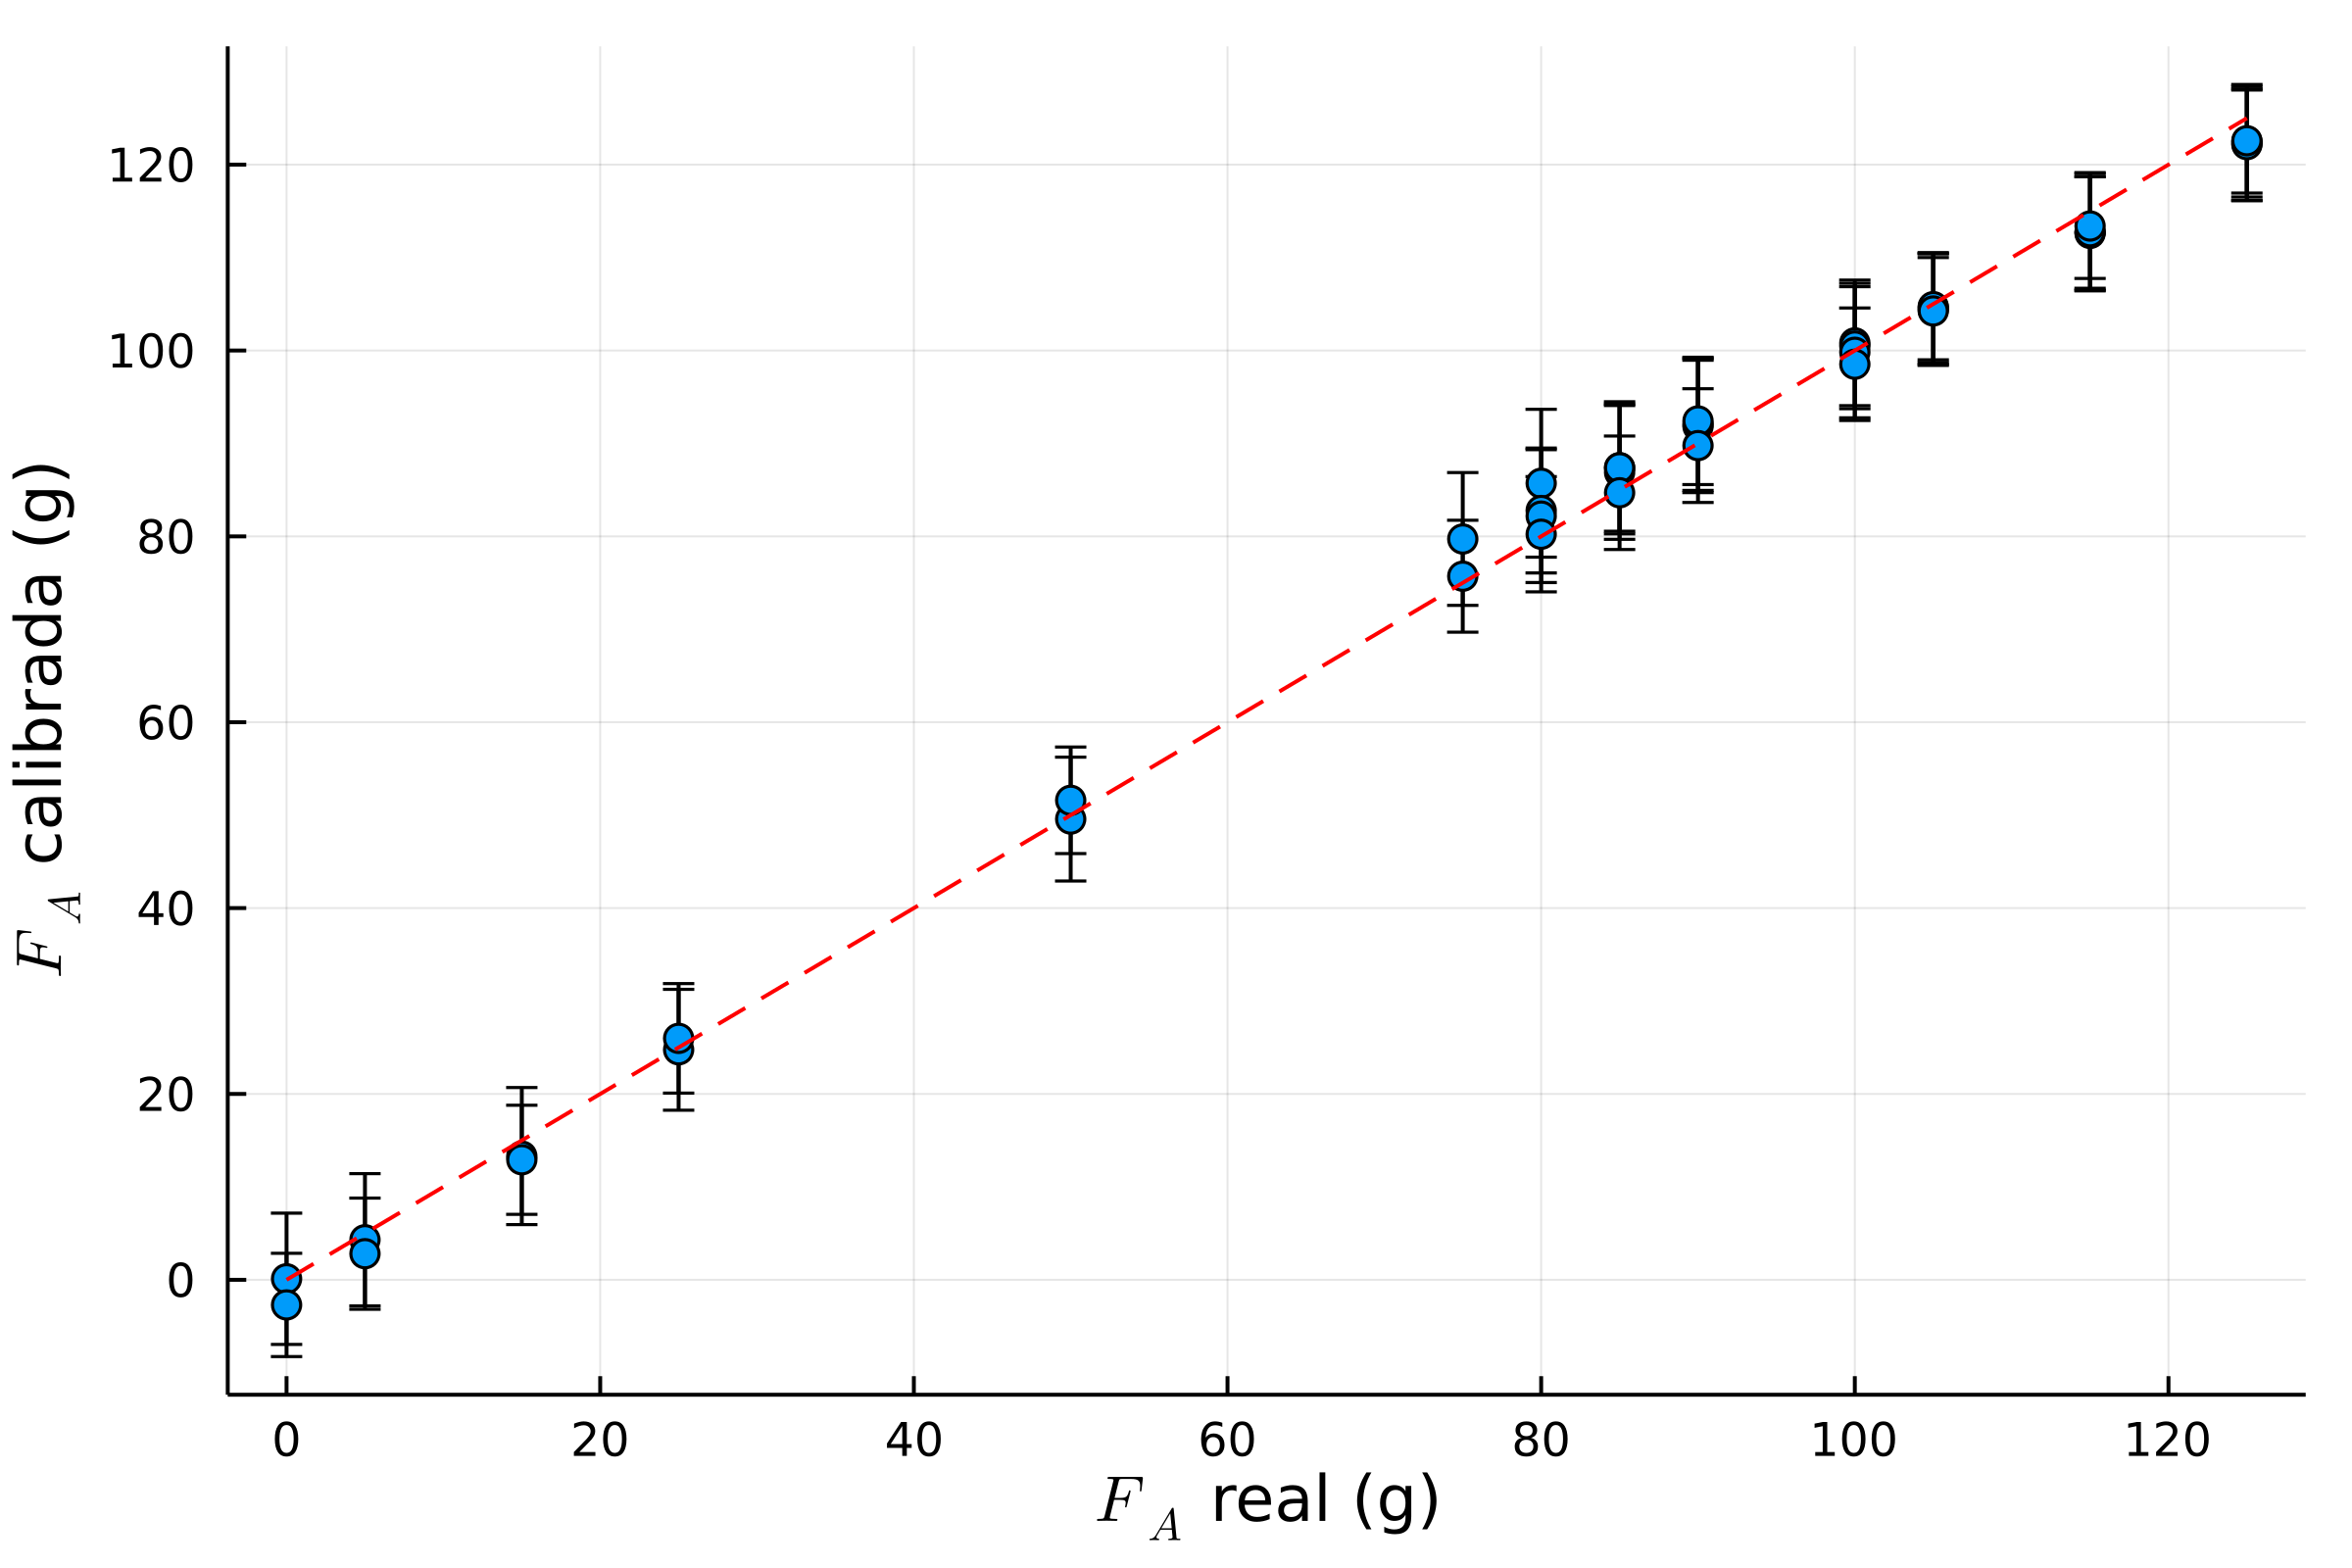
\includegraphics[height=.29\textheight]{img/results/calibration_FA.png}
        \caption{Componente \textit{aft}.}\label{fig:calibration_FA}
    \end{subfigure}
    \begin{subfigure}{\textwidth}\centering
        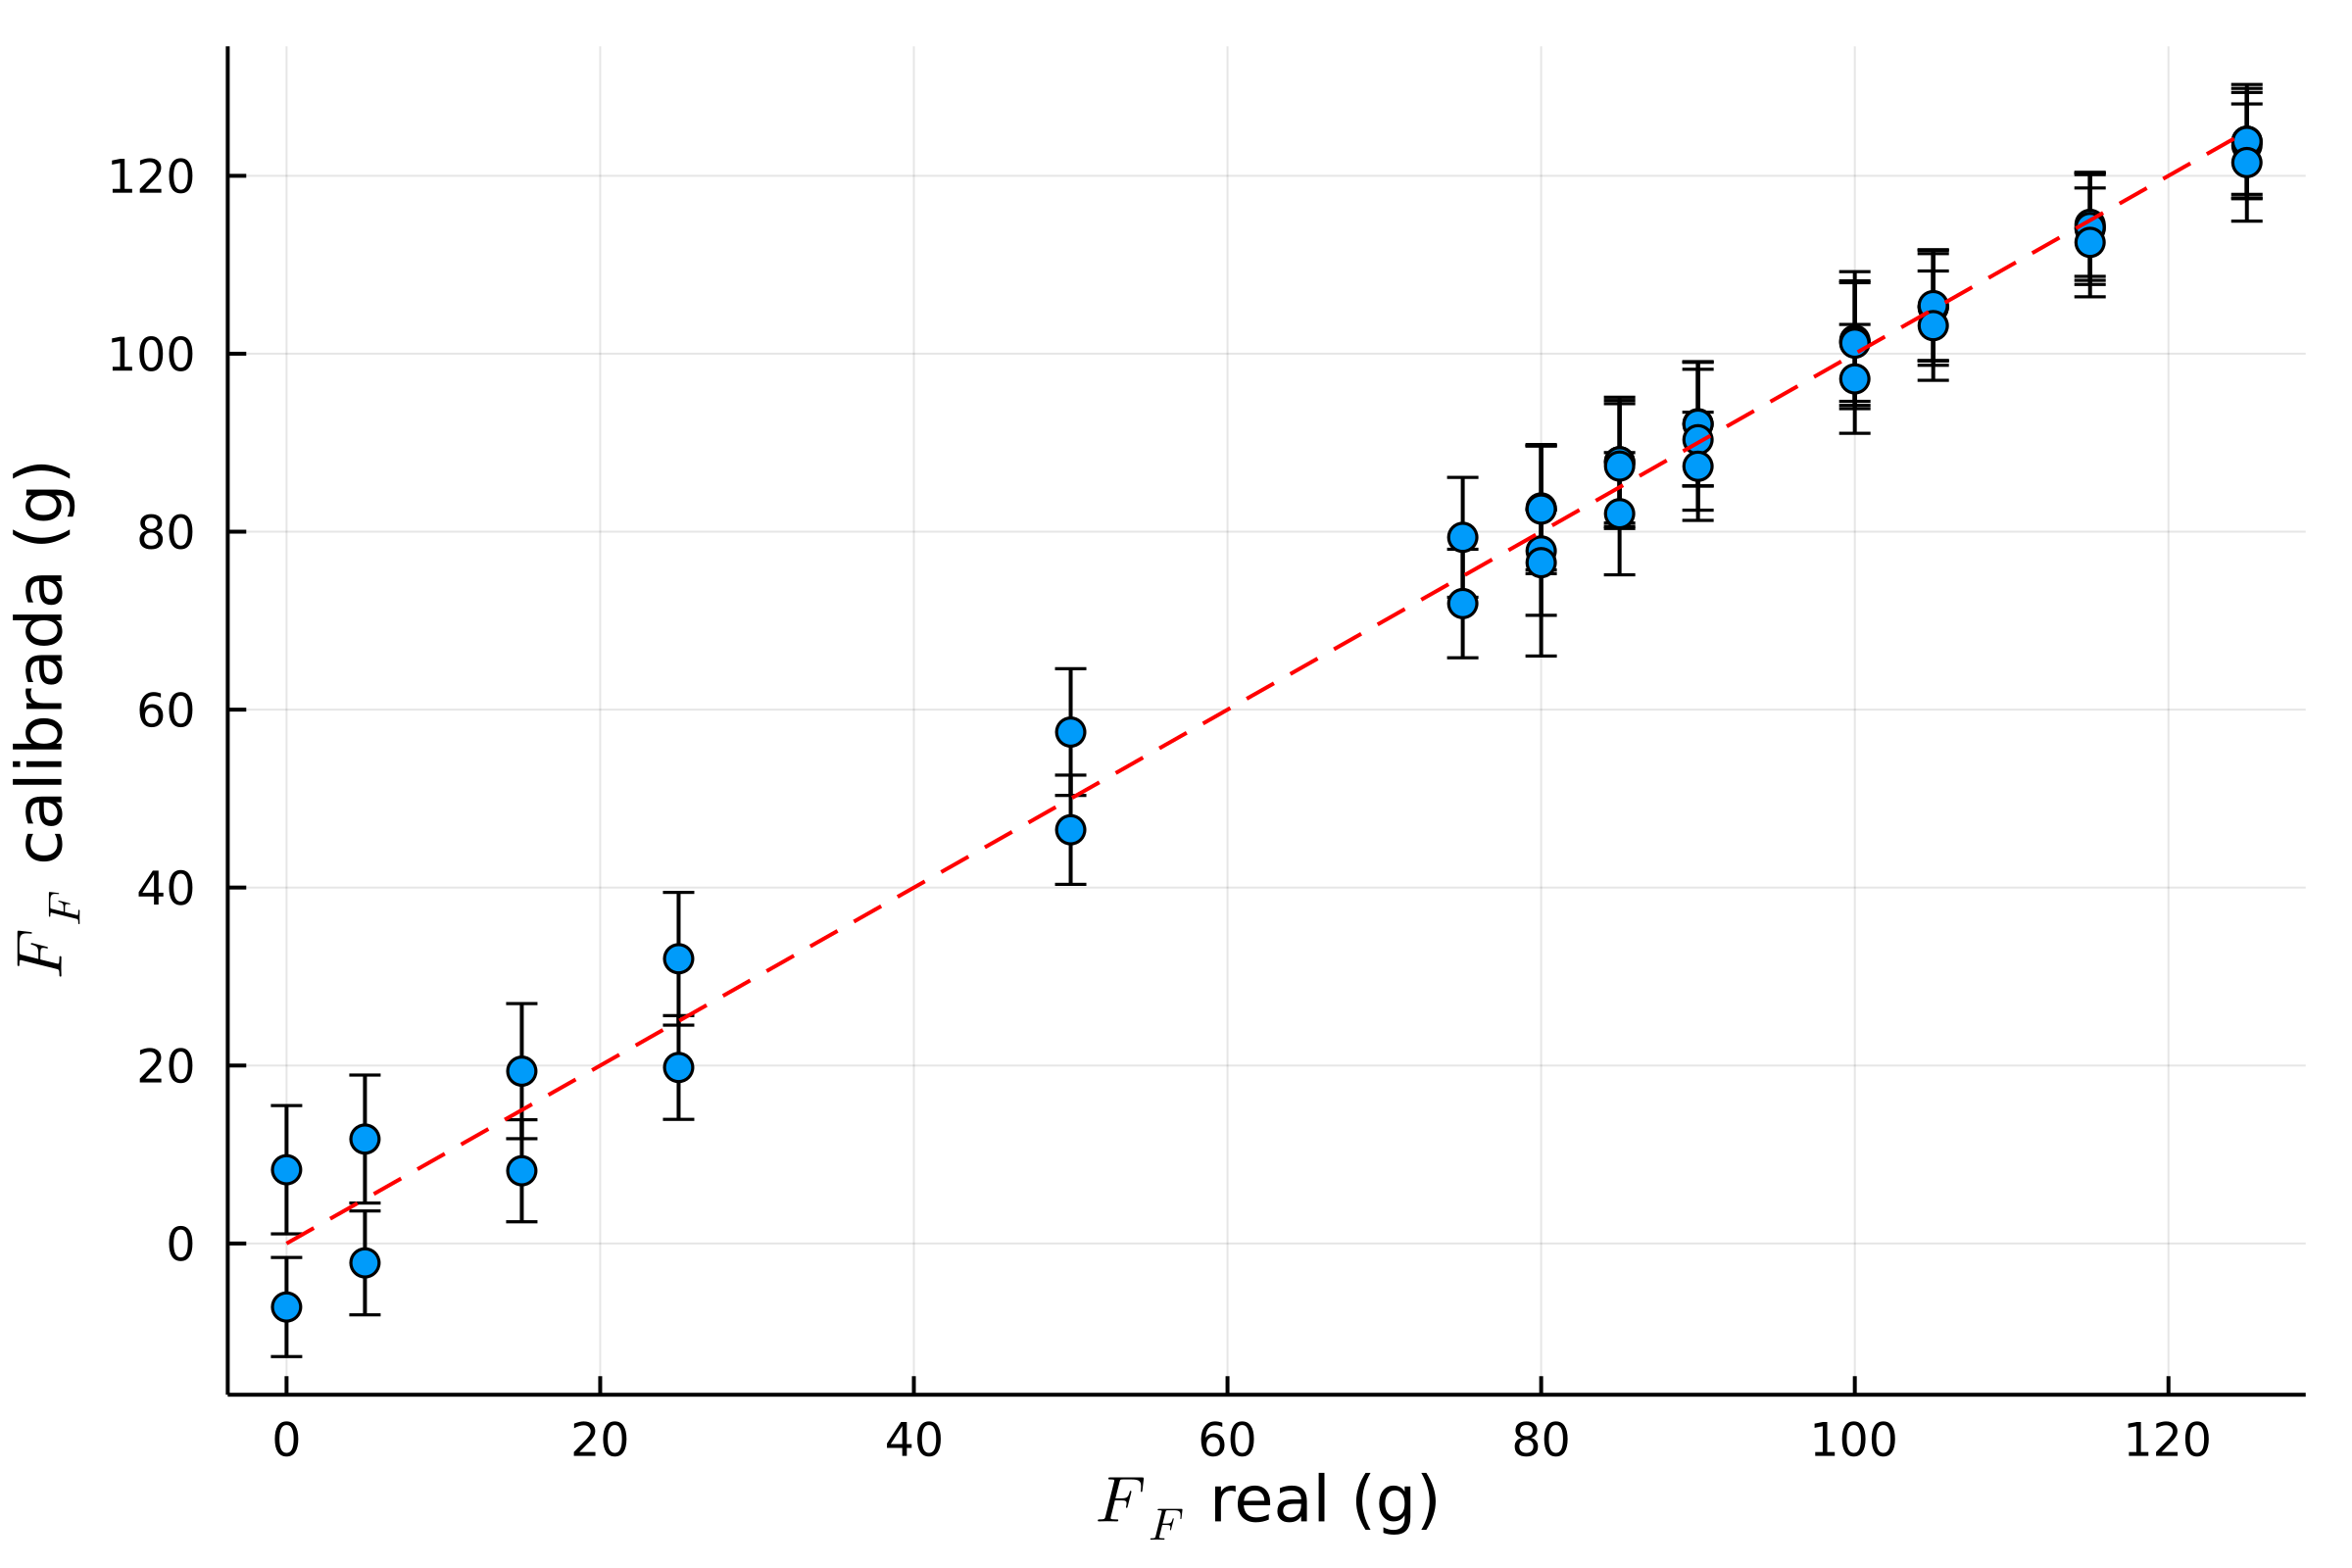
\includegraphics[height=.29\textheight]{img/results/calibration_FF.png}
        \caption{Componente \textit{fore}.}\label{fig:calibration_FF}
    \end{subfigure}
    \begin{subfigure}{\textwidth}\centering
        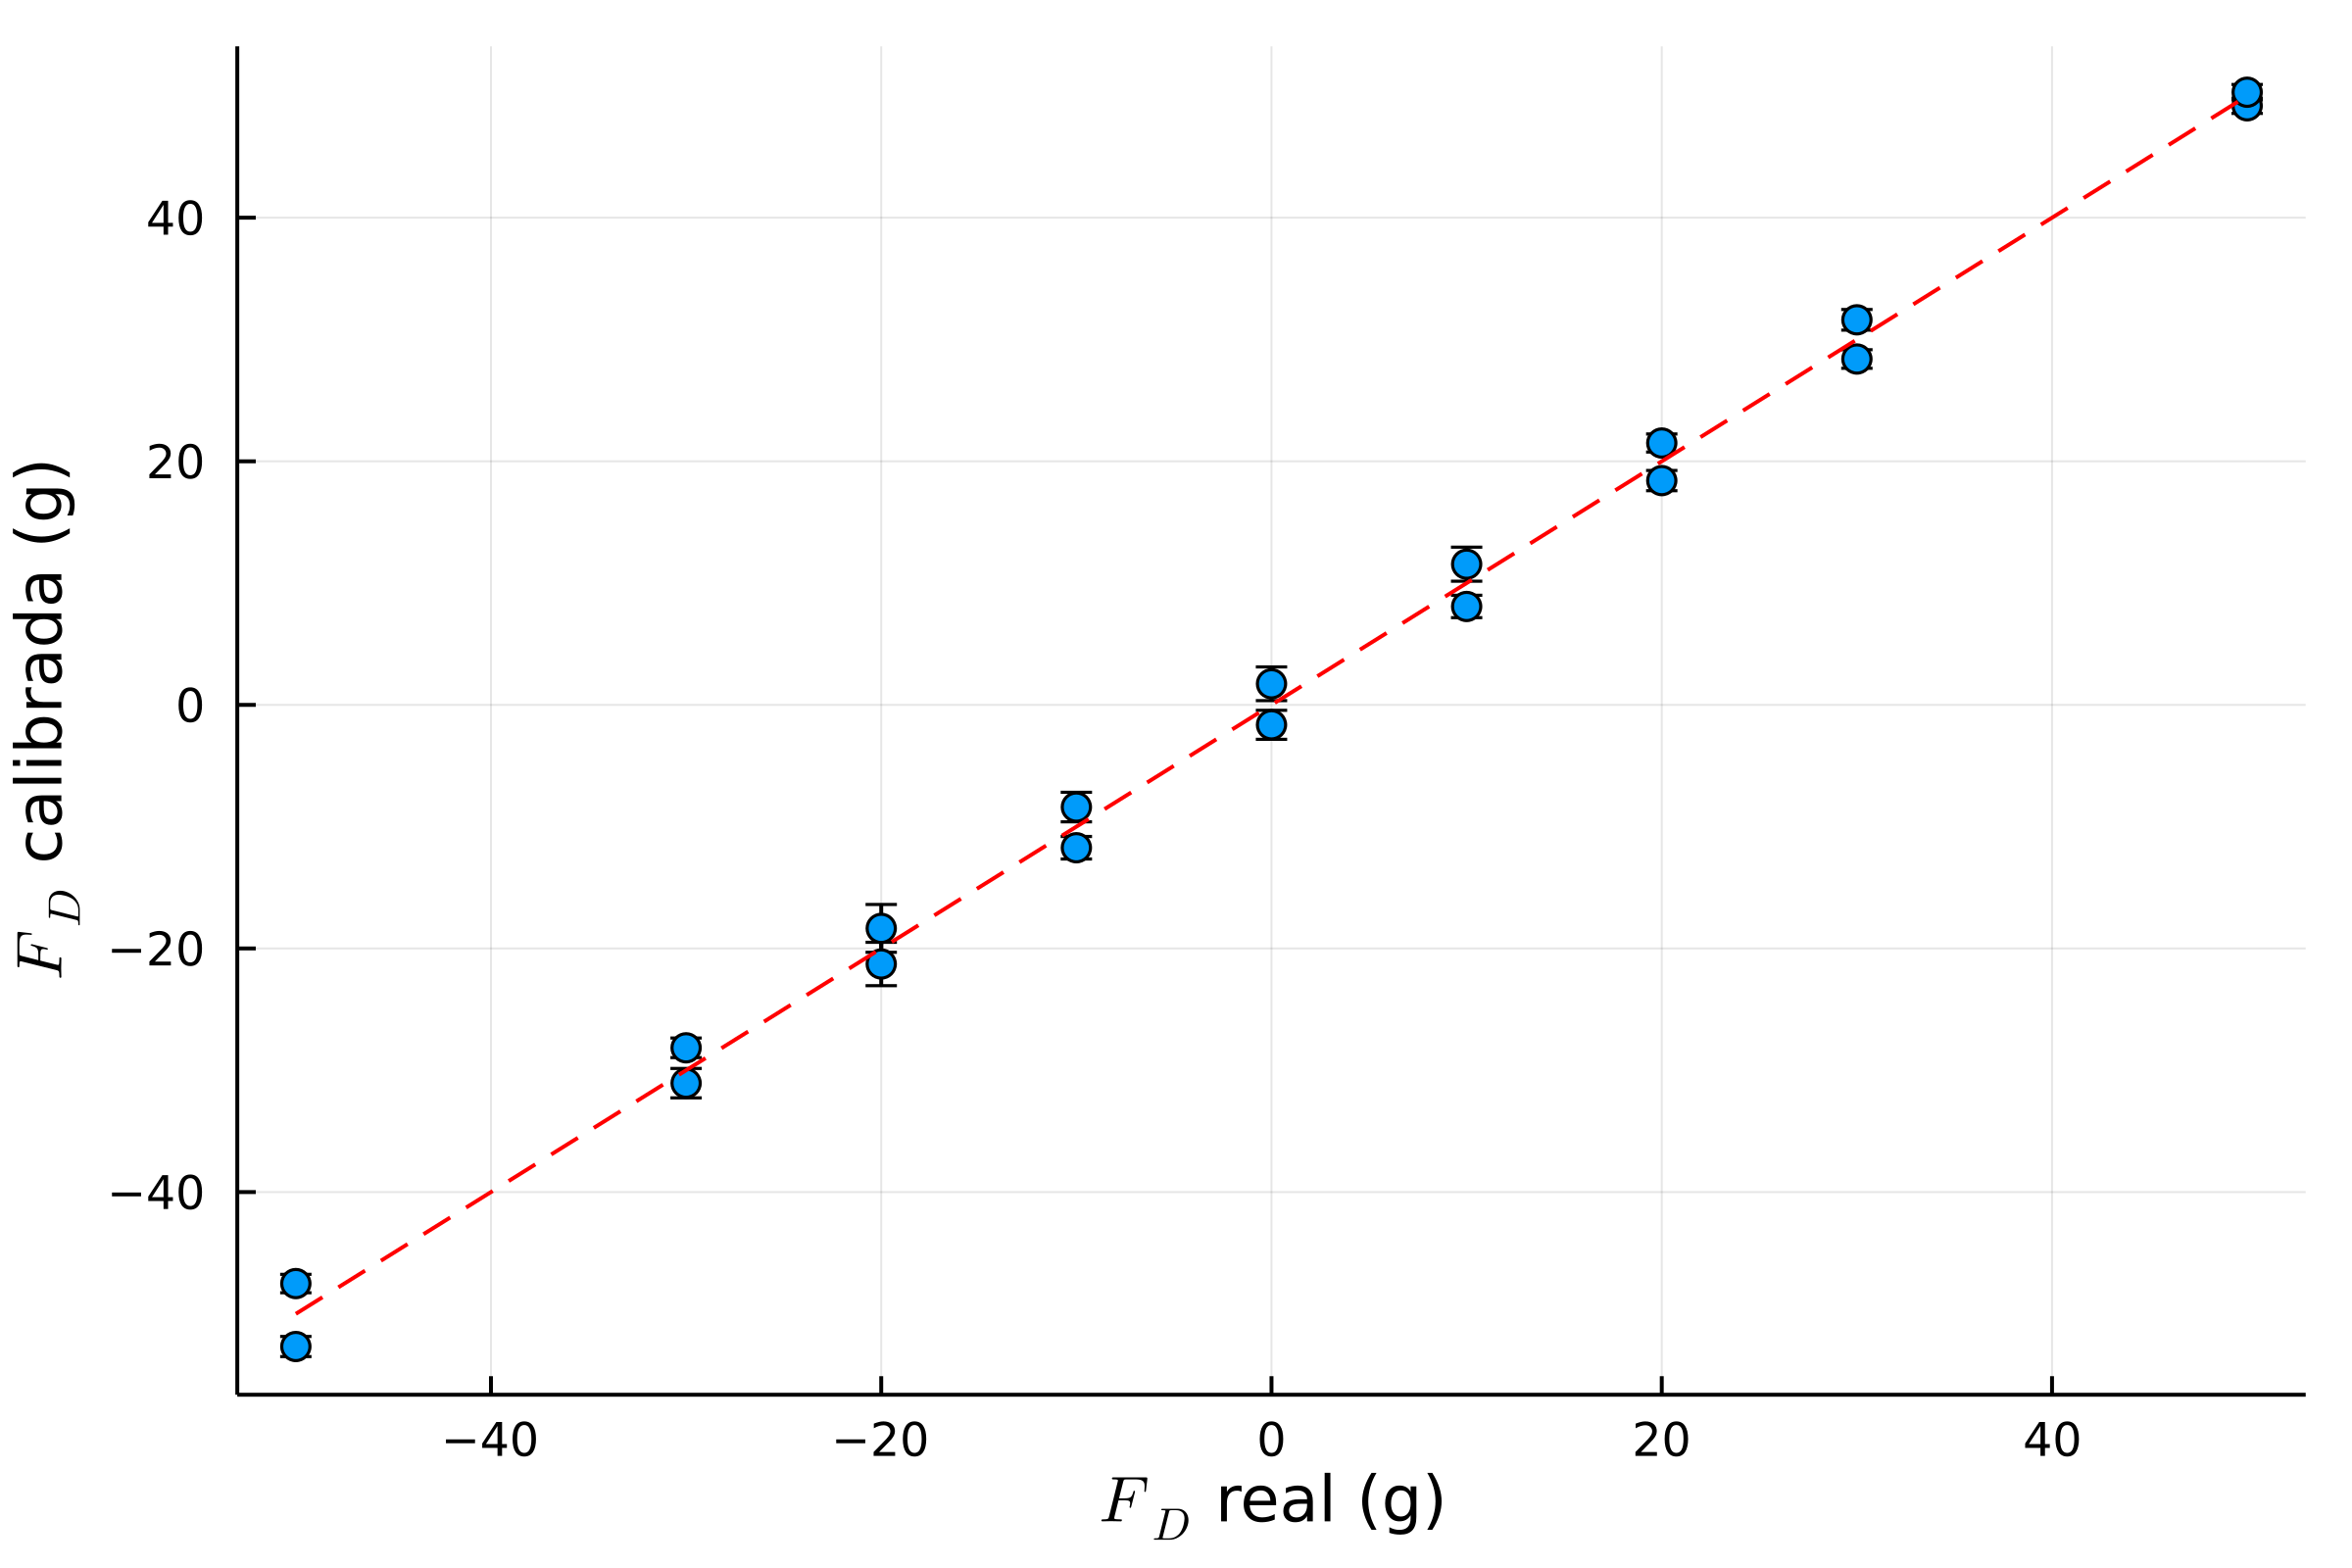
\includegraphics[height=.29\textheight]{img/results/calibration_FD.png}
        \caption{Componente \textit{drag}.}\label{fig:calibration_FD}
    \end{subfigure}
    \caption{Curvas de calibração dos componentes da balança.}\label{fig:calibration_curves}
\end{figure}

Os resultados de empuxo sem lâmina defletora estão exibidos na figura~\ref{fig:thrust_no_deflector}. A primeira linha vermelha tracejada, à esquerda, indica o acionamento do compressor de ar. A segunda, indica seu desligamento, e por fim a terceira seu acionamento final. O compressor de ar usado aciona-se automaticamente quando a pressão do reservatório (400L) reduz-se abaixo de certo limite (8bar). Assim, esse experimento demonstra que as variações de pressão no reservatório pouco afetam o experimento, conectado ao reservatório de ar por uma válvula reguladora. A queda de empuxo ao final do experimento ocorreu após quase um minuto de coleta de dados, de modo que foi comprovada a capacidade de fornecimento de ar do compressor. Com estes dados, e também o valor do coeficiente de empuxo empírico, conclui-se que a pressão real de câmara obtida foi de \(5,60\pm 0,15\;\mathrm{bar}\). A diferença deste valor para os valores obtidos no gráfico~\ref{fig:thrust_versus_p1} deve-se à mudança do sistema de compressão de ar utilizado.

\begin{figure}[htbp]
    \centering
    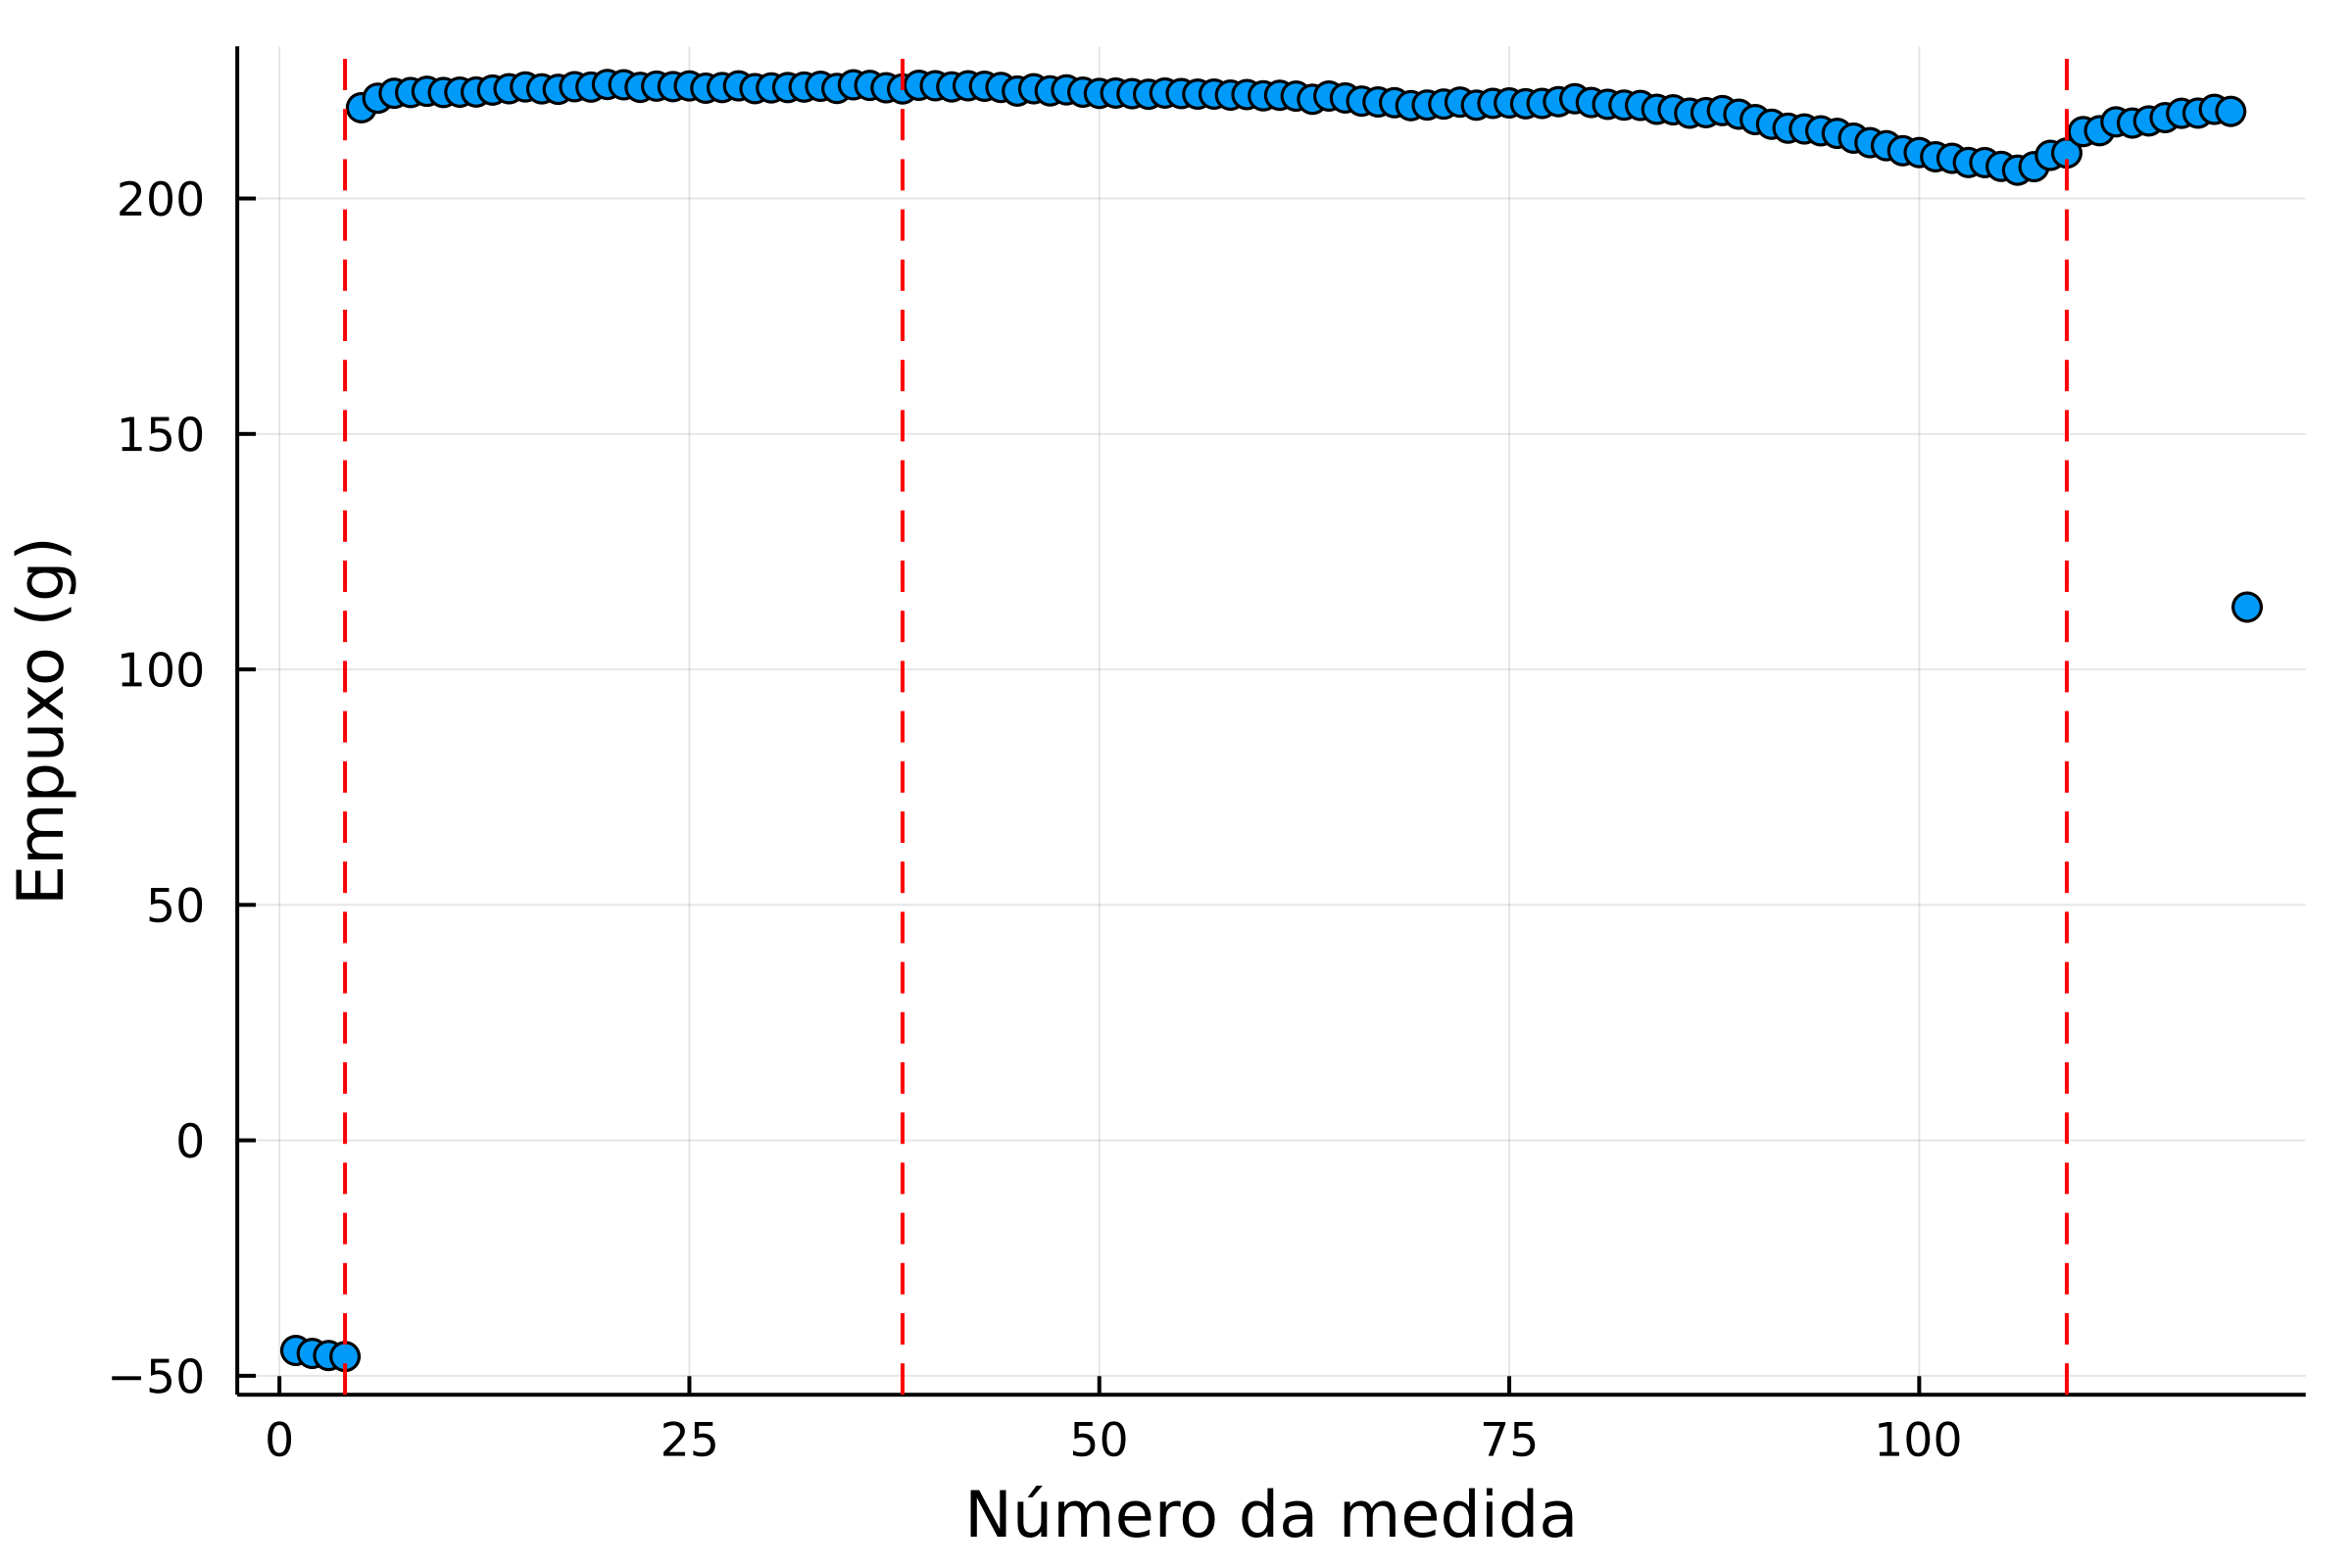
\includegraphics[width=\textwidth]{img/results/thrust_no_deflector.png}
    \caption{Medidas de empuxo sem lâmina defletora.}\label{fig:thrust_no_deflector}
\end{figure}

Finalmente, apresentam-se os gráficos de forças e momento em função da deflexão do servomotor. Recorda-se aqui que a posição de \(90\mathrm{^{\circ}}\) do servomotor corresponde ao paralelismo da lâmina defletora com o escoamento da tubeira. Como mencionado na seção~\ref{sec:method_3axis_measurement}, foram feitas três repetições de varreduras crescentes e decrescentes de posição. Os gráficos de \(F_x\), \(F_y\) e \(M\) obtidos após conversão das saídas dos componentes para forças aplicadas (através da calibração e equações~\ref{eq:FA} a~\ref{eq:FD}) estão exibidos na figura~\ref{fig:deflection_forces}.

\begin{figure}[htbp]
    \centering
    \begin{subfigure}{0.49\textwidth}
        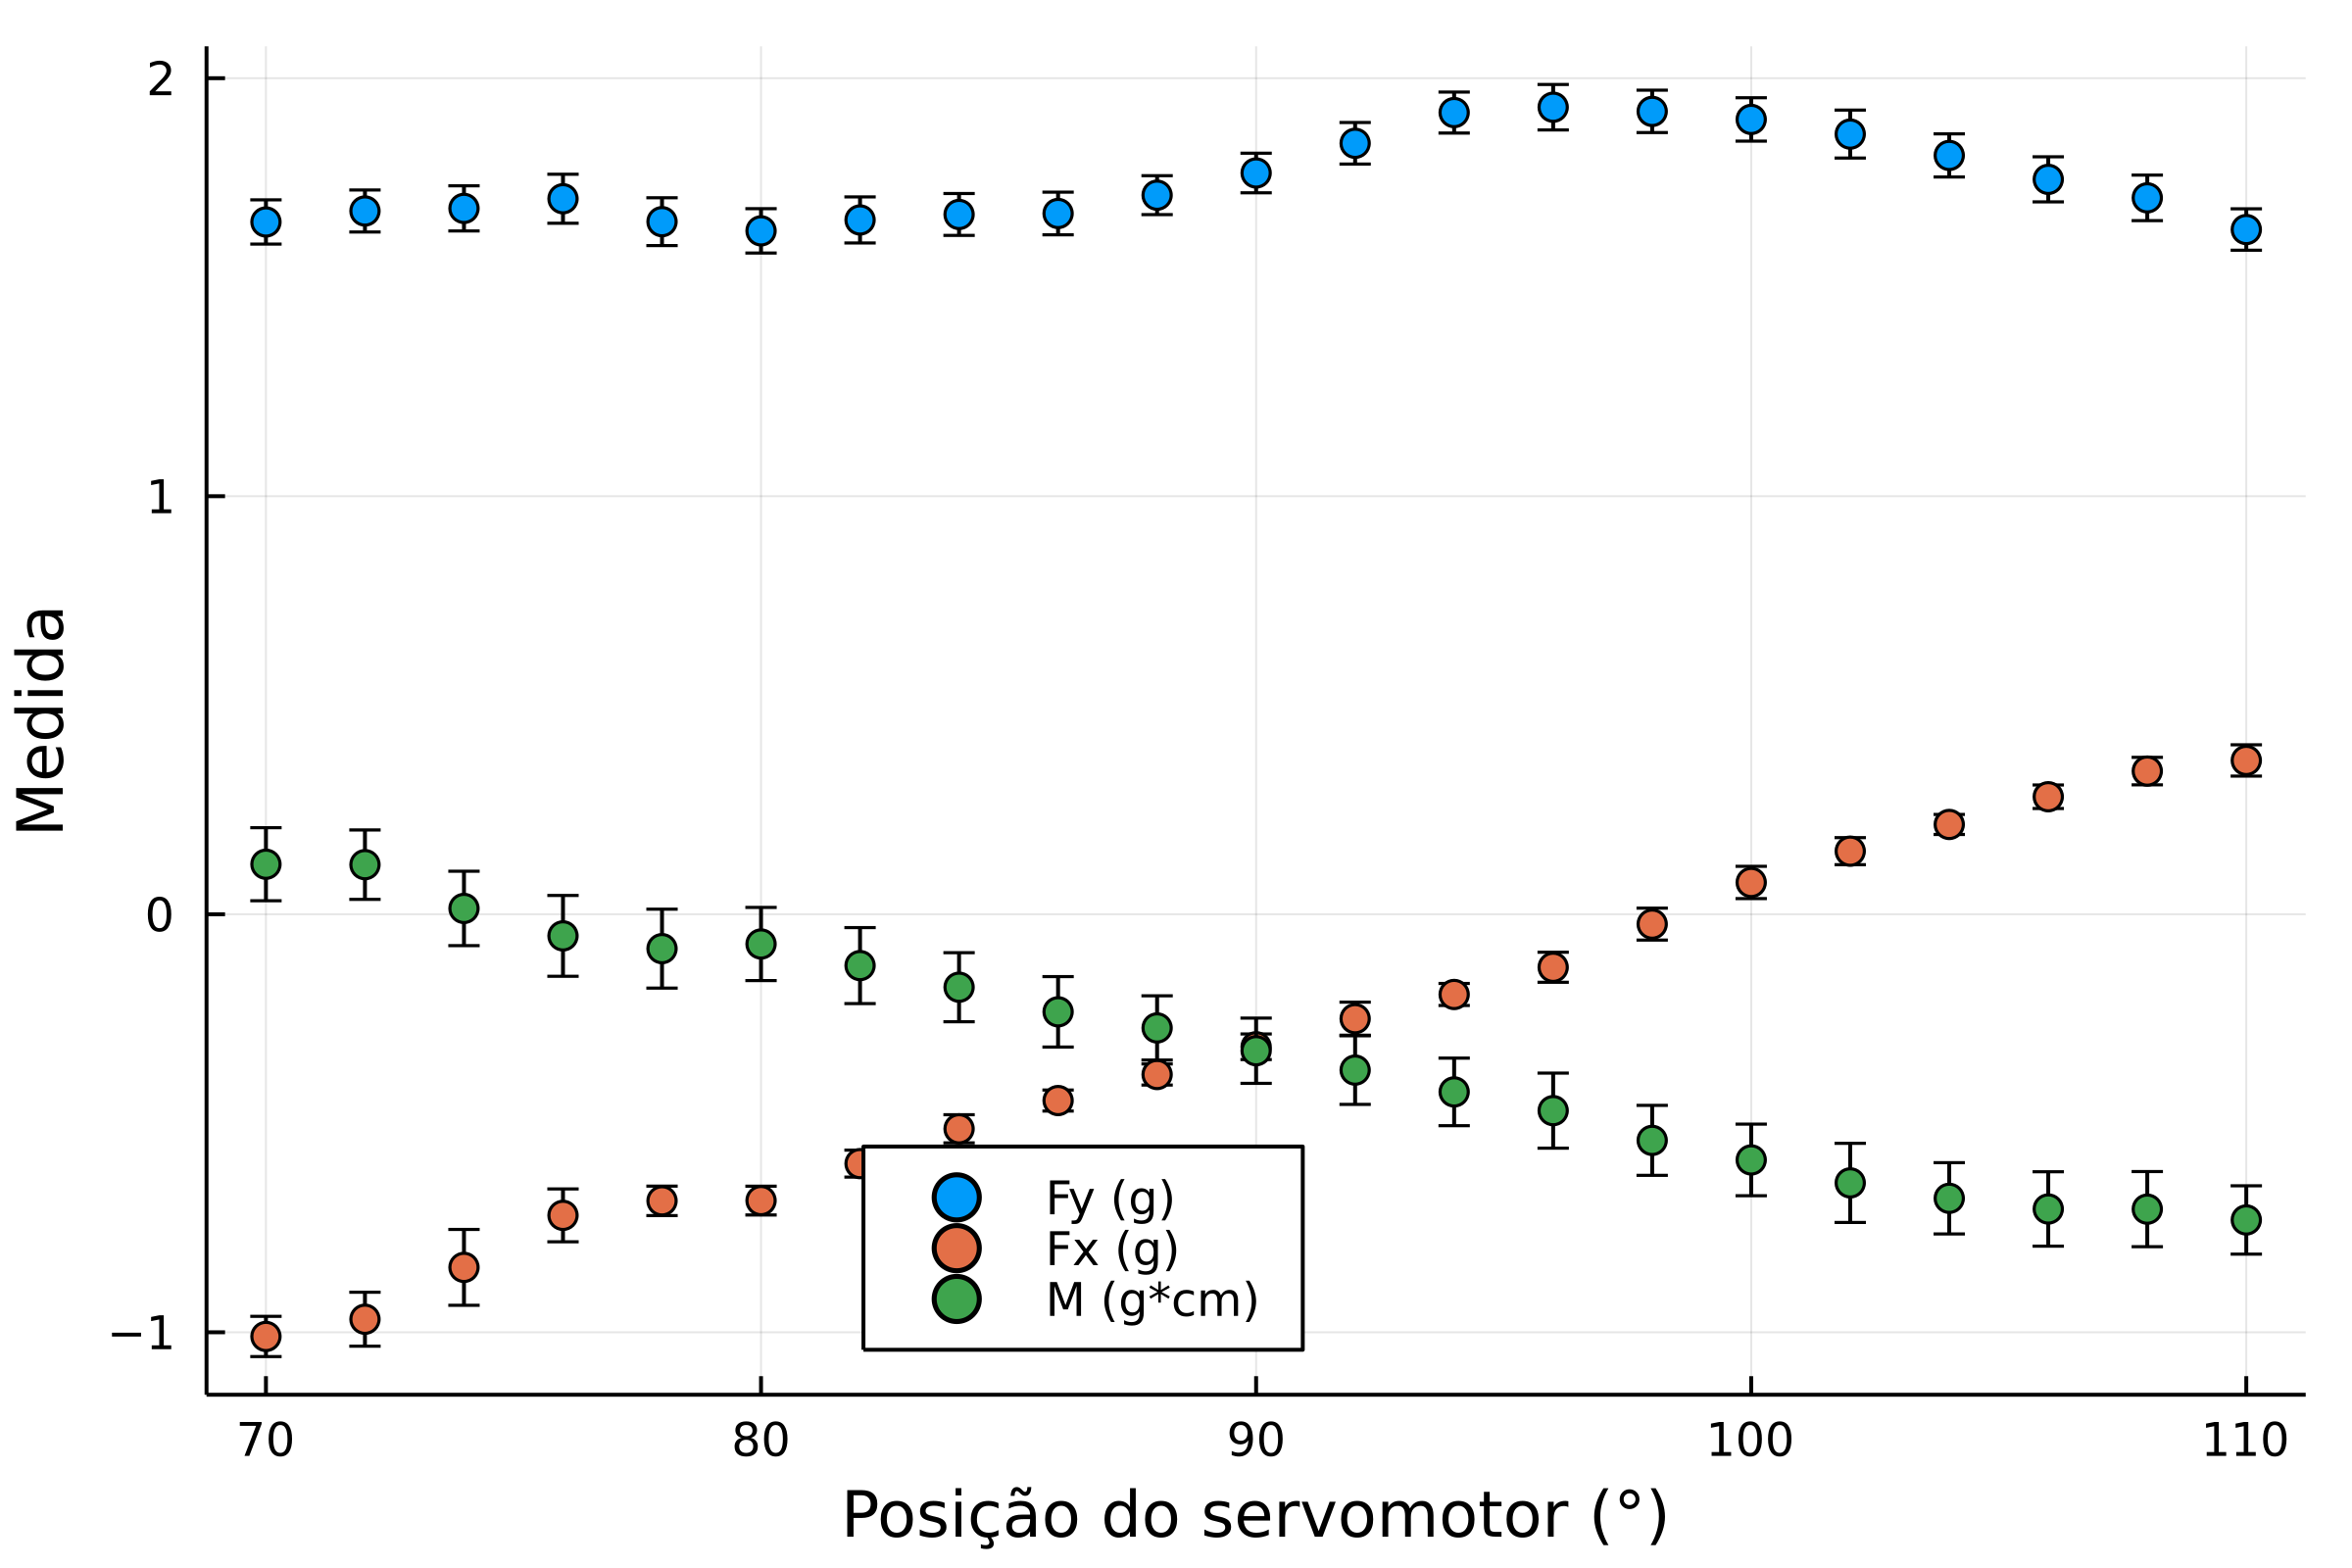
\includegraphics[width=\textwidth]{img/results/exp7_5bar_70_a_110.png}
    \end{subfigure}
    \begin{subfigure}{0.49\textwidth}
        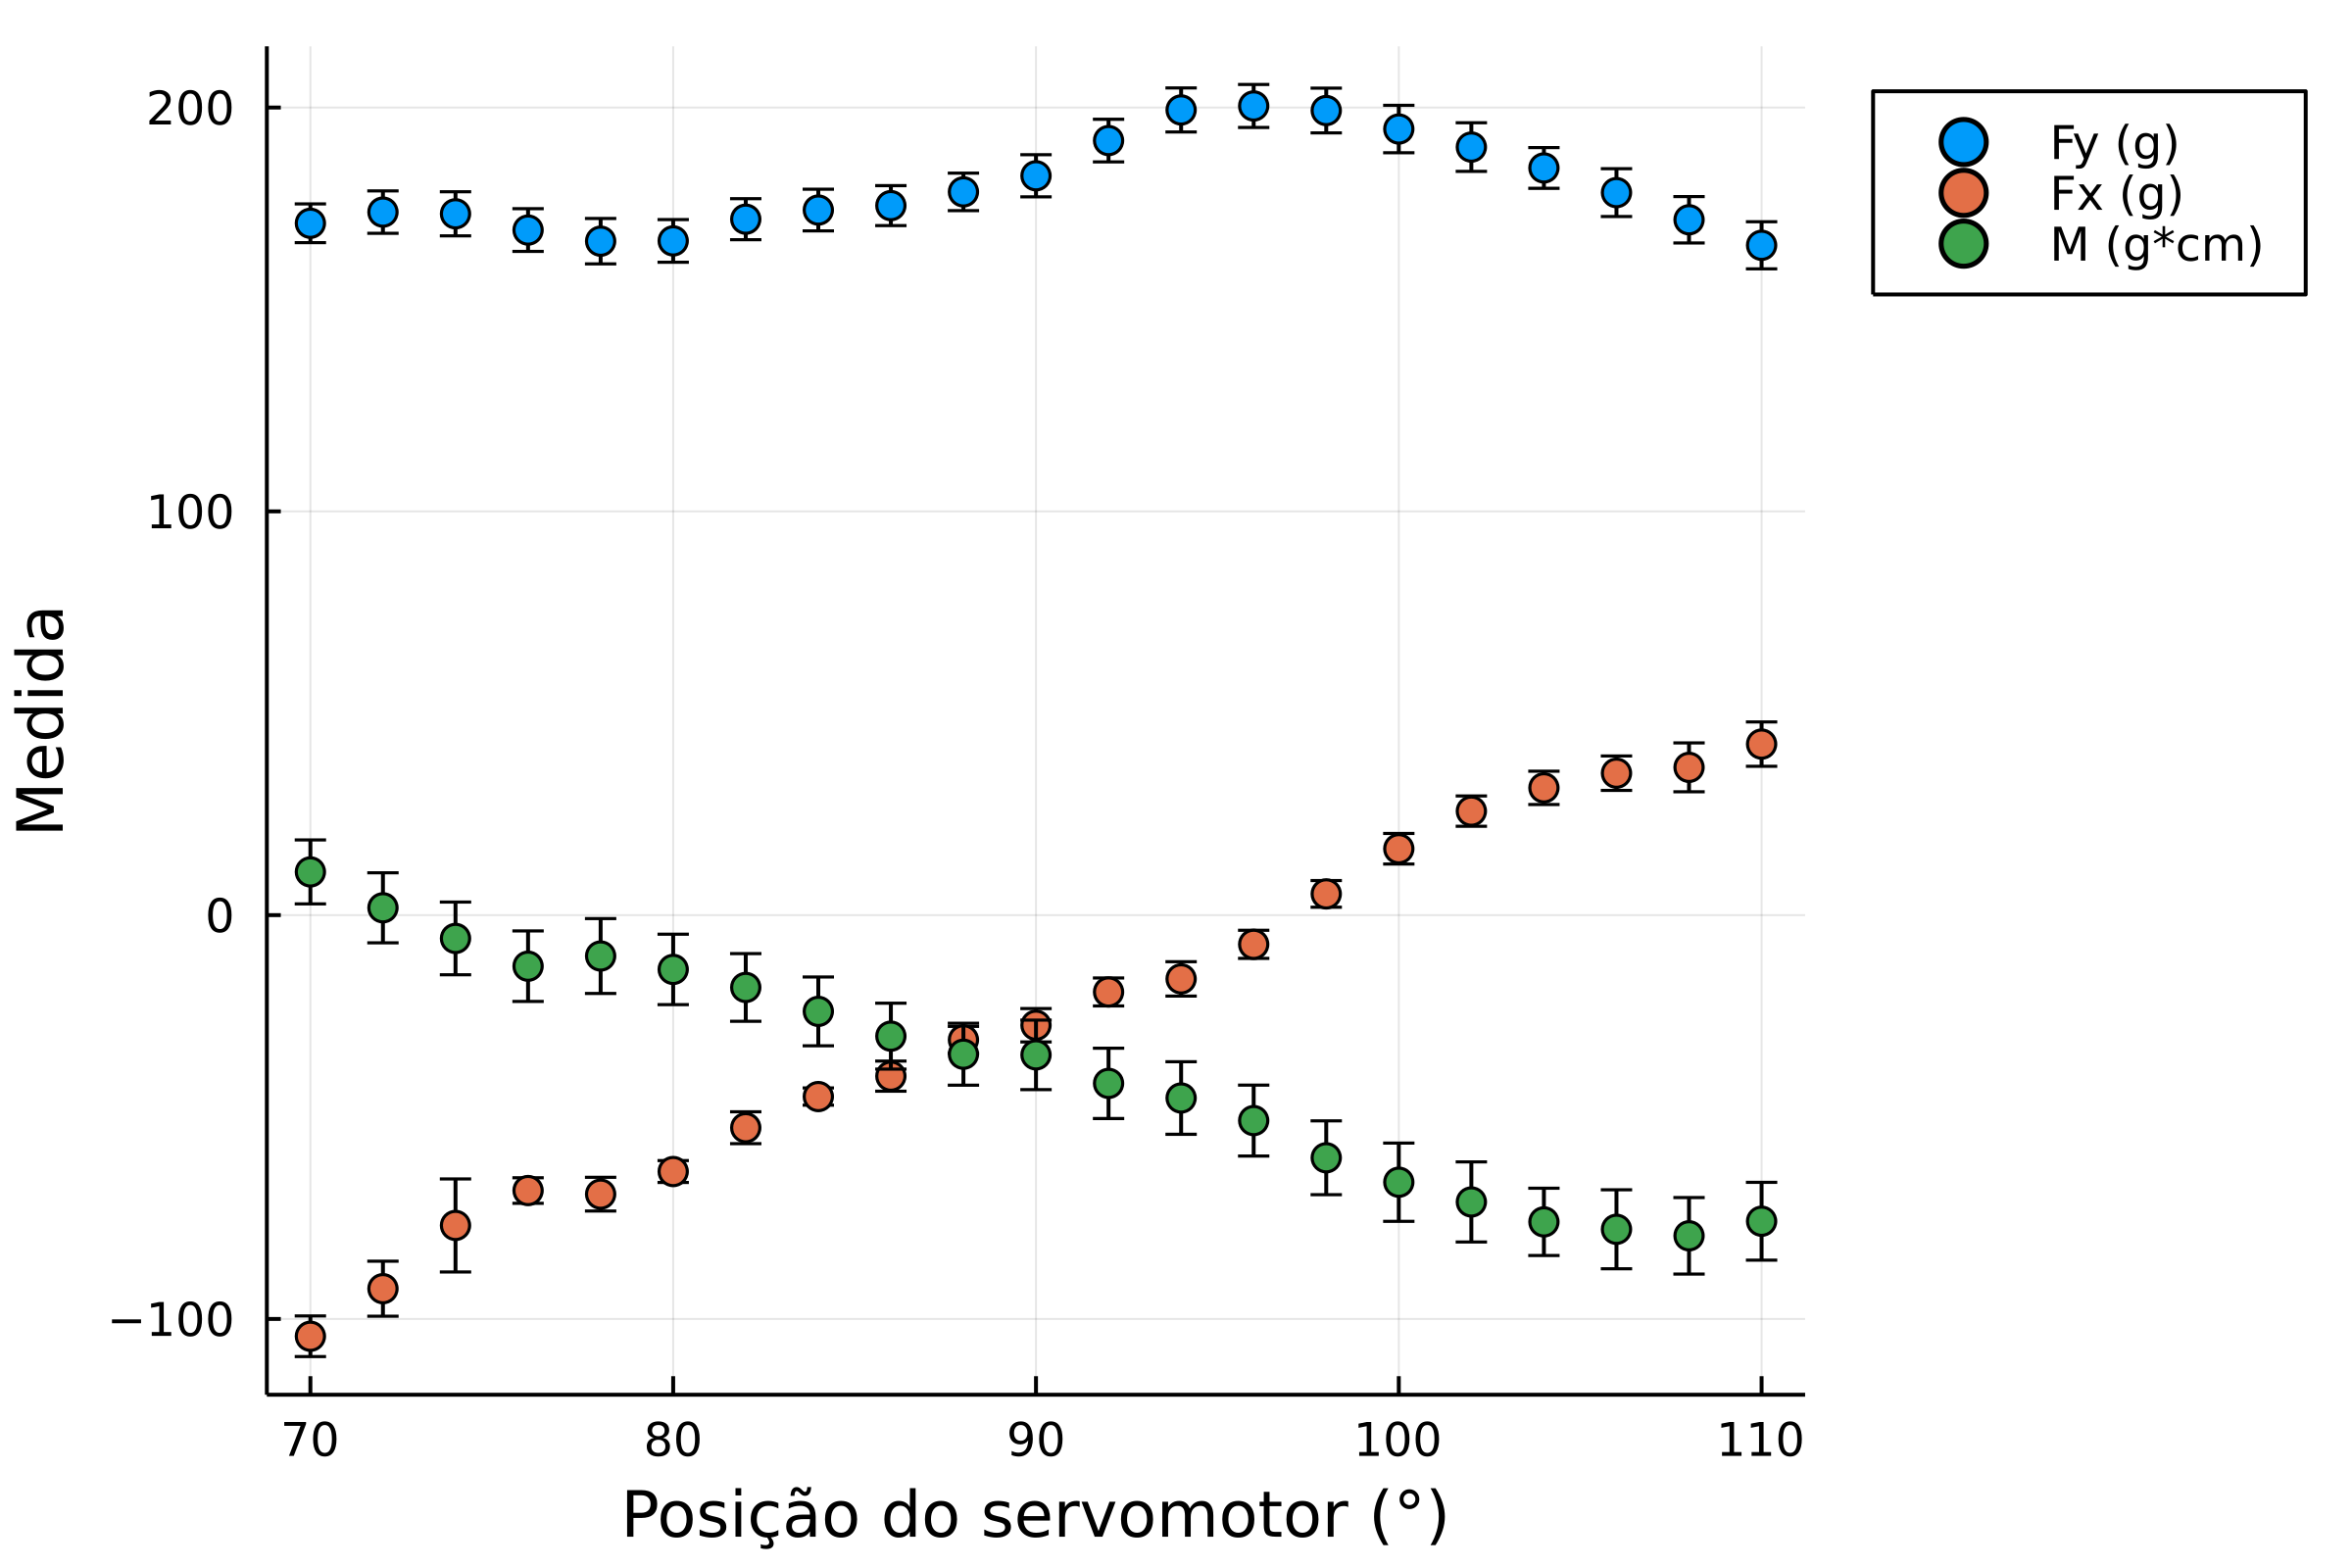
\includegraphics[width=\textwidth]{img/results/exp8_5bar_110_a_70.png}
    \end{subfigure}
    \begin{subfigure}{0.49\textwidth}
        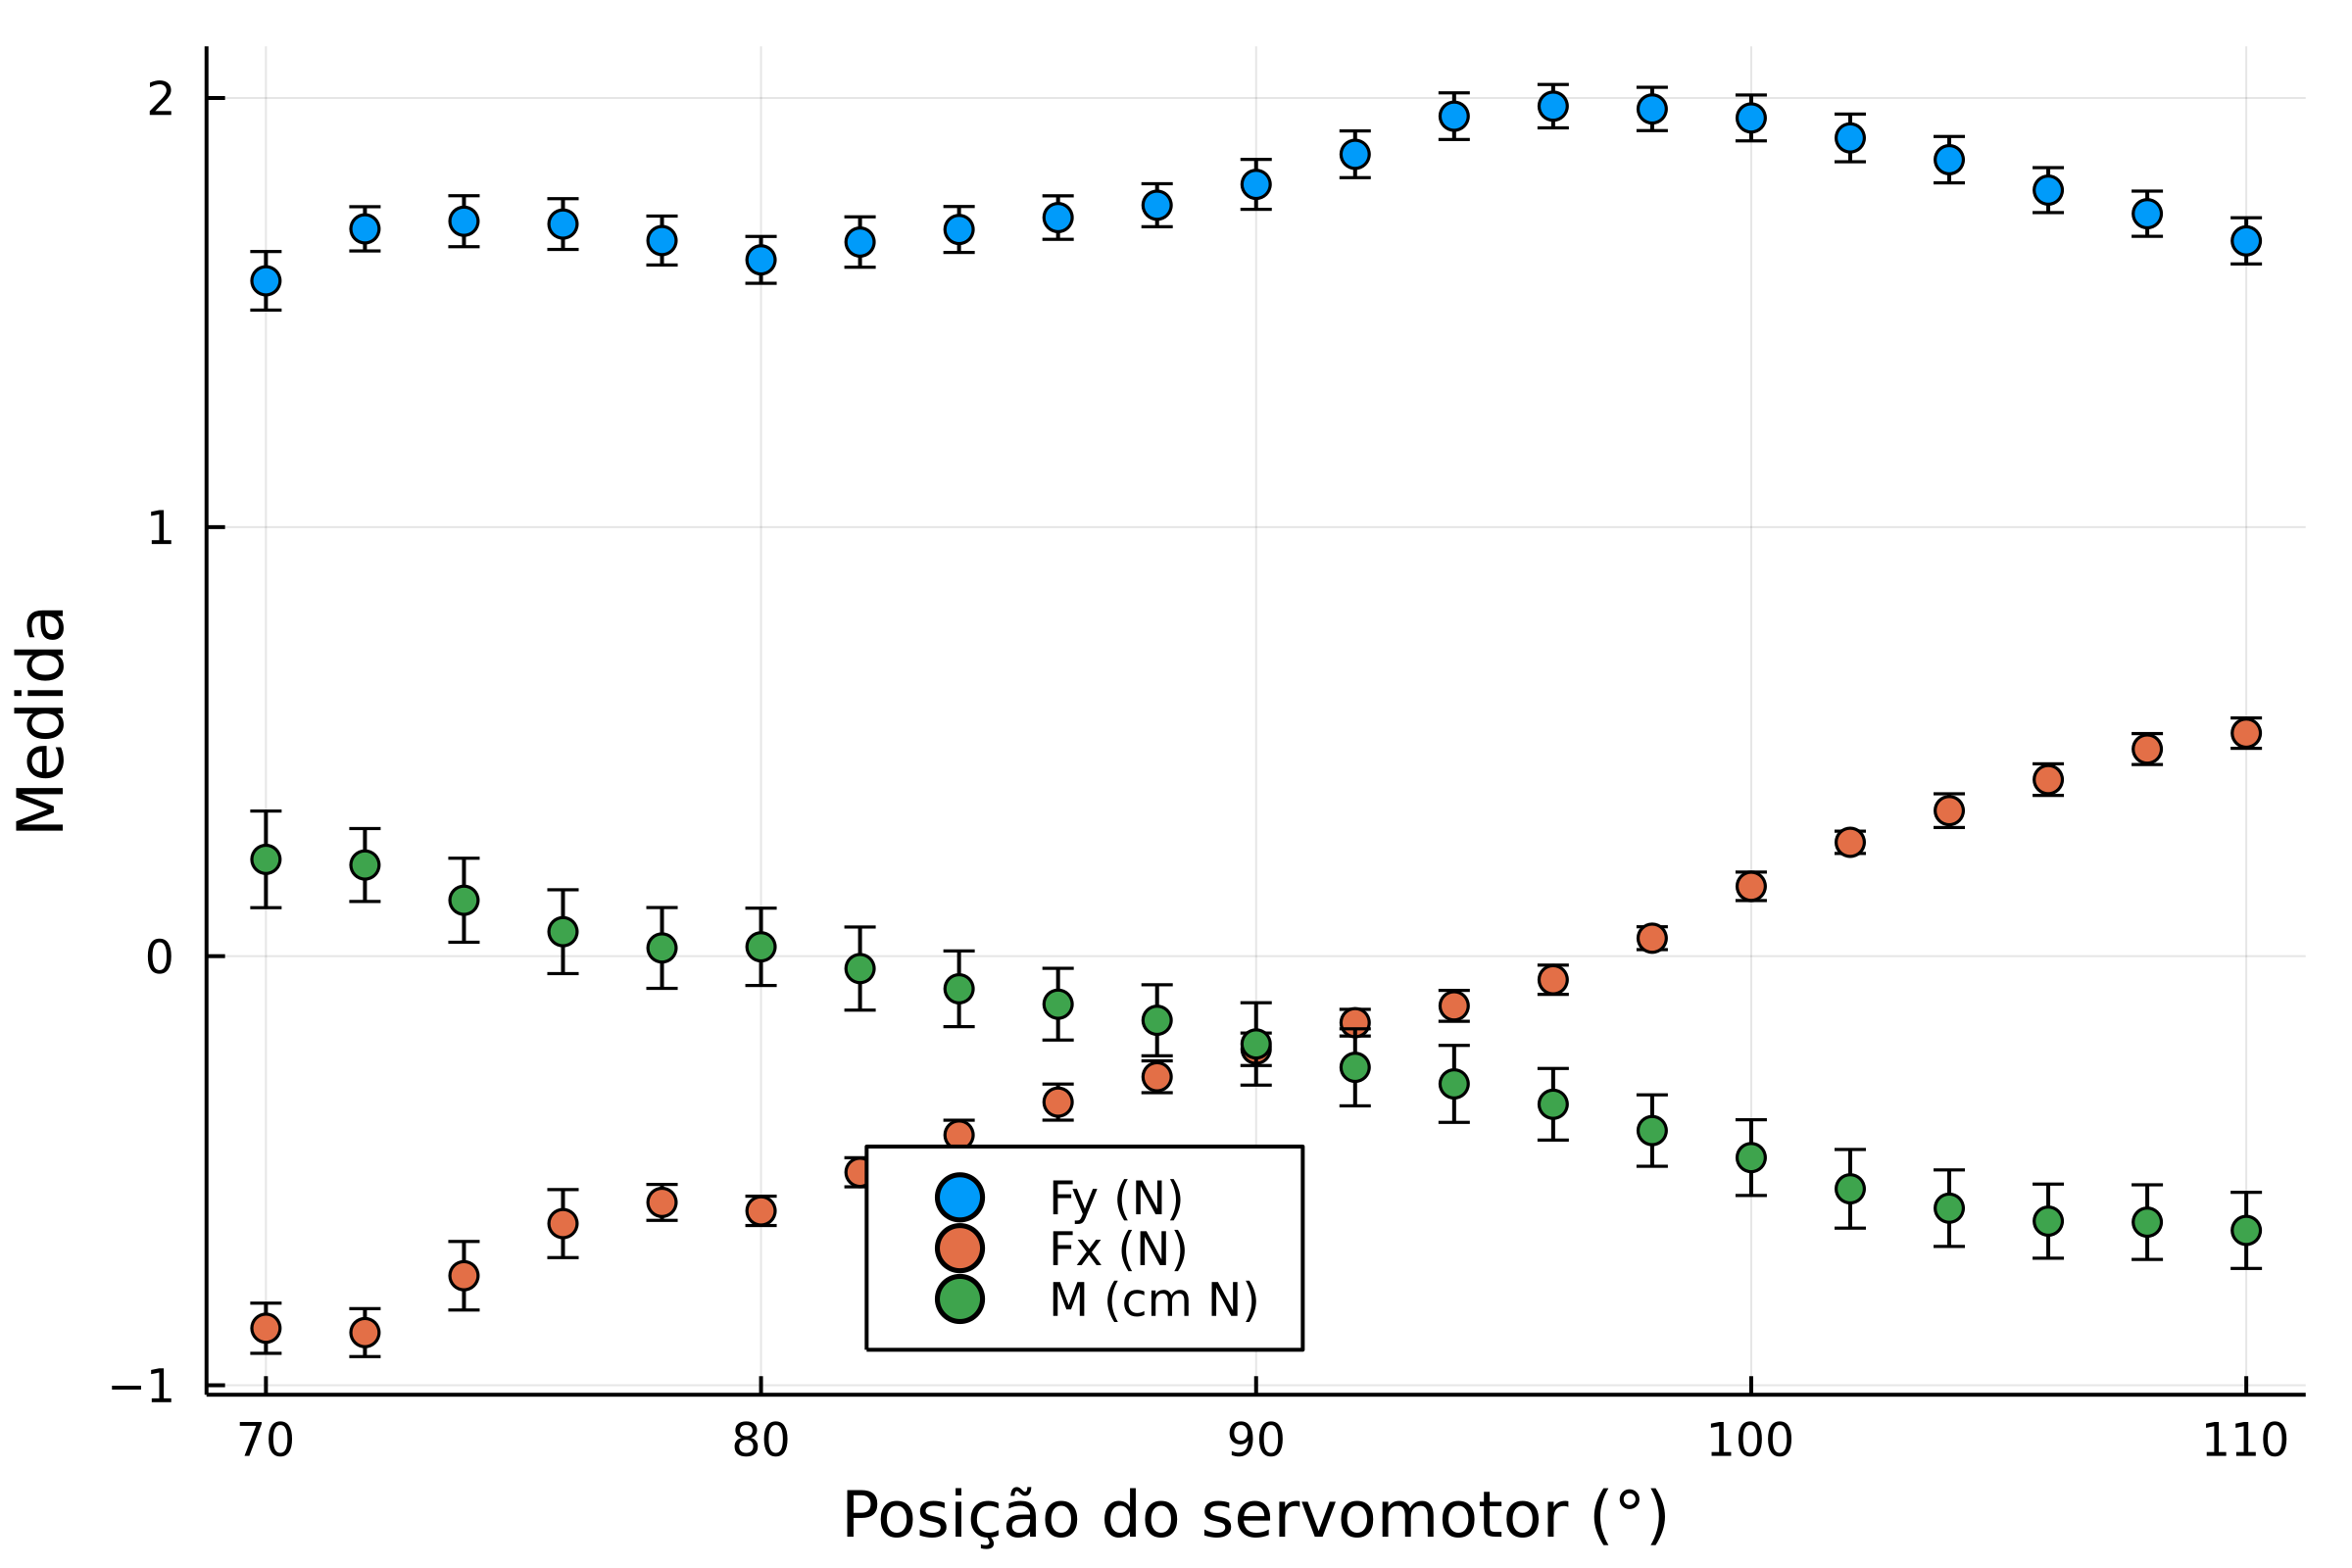
\includegraphics[width=\textwidth]{img/results/exp9_5bar_70_a_110.png}
    \end{subfigure}
    \begin{subfigure}{0.49\textwidth}
        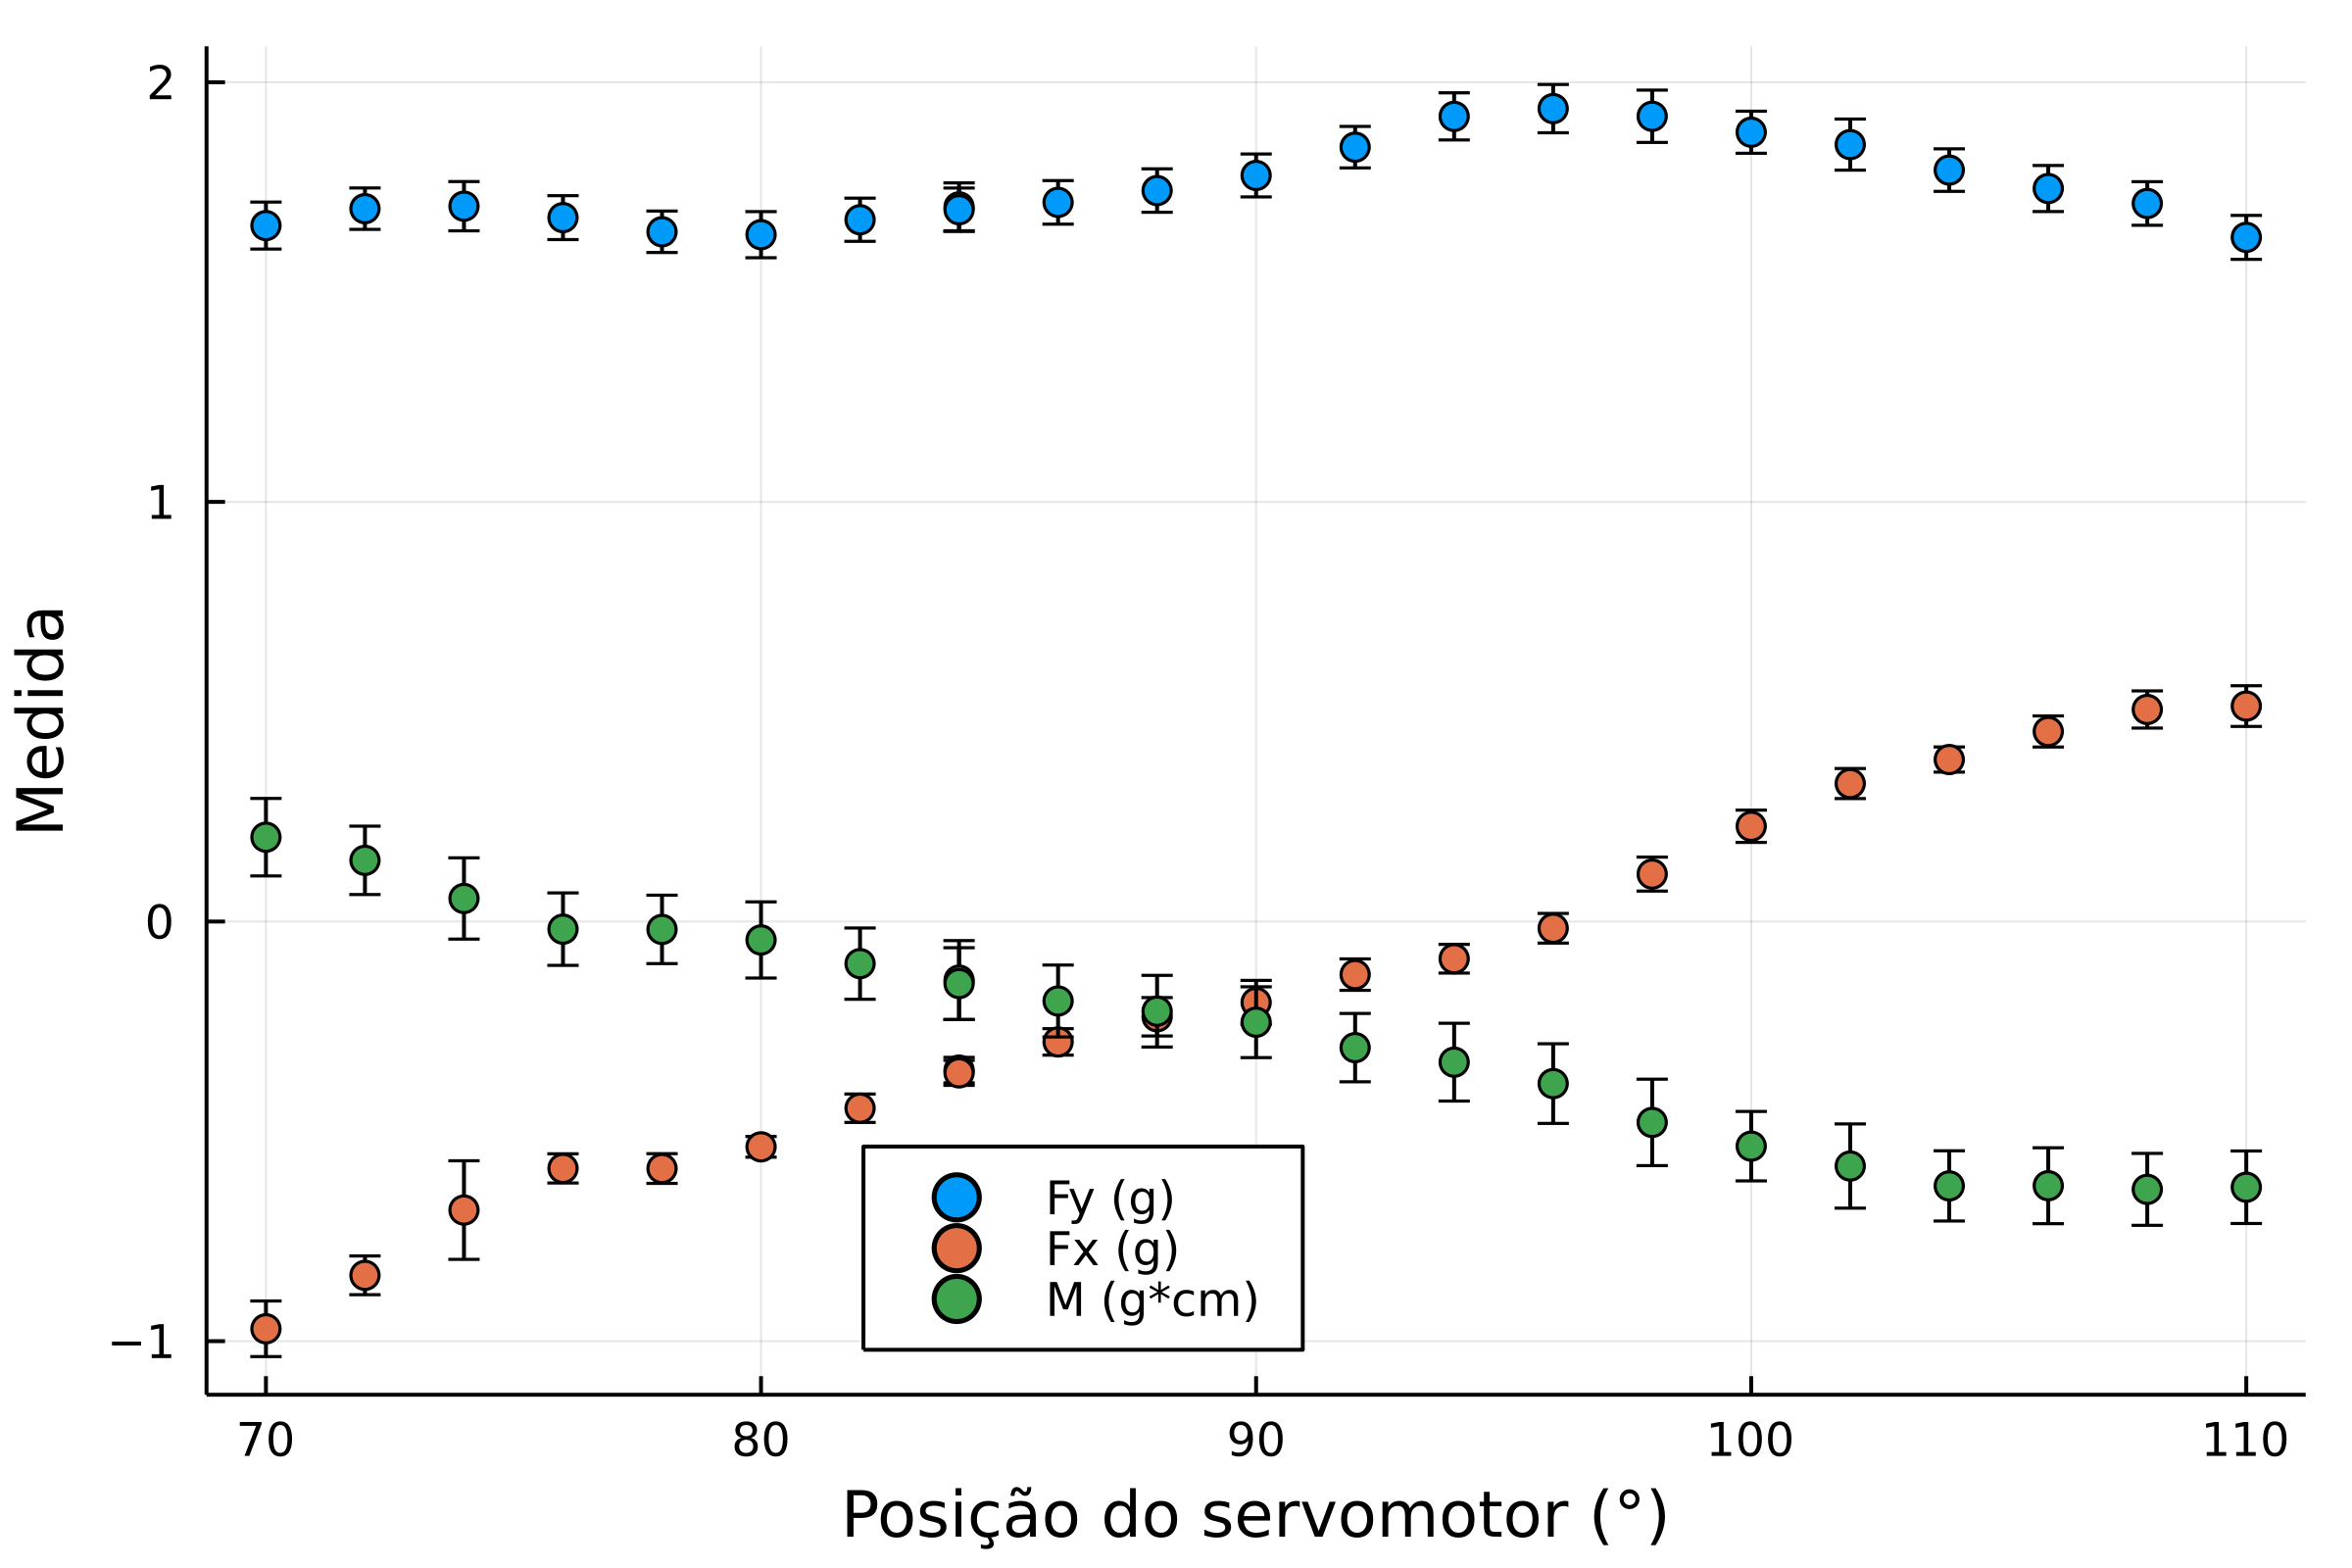
\includegraphics[width=\textwidth]{img/results/exp10_5bar_110_a_70.png}
    \end{subfigure}
    \begin{subfigure}{0.49\textwidth}
        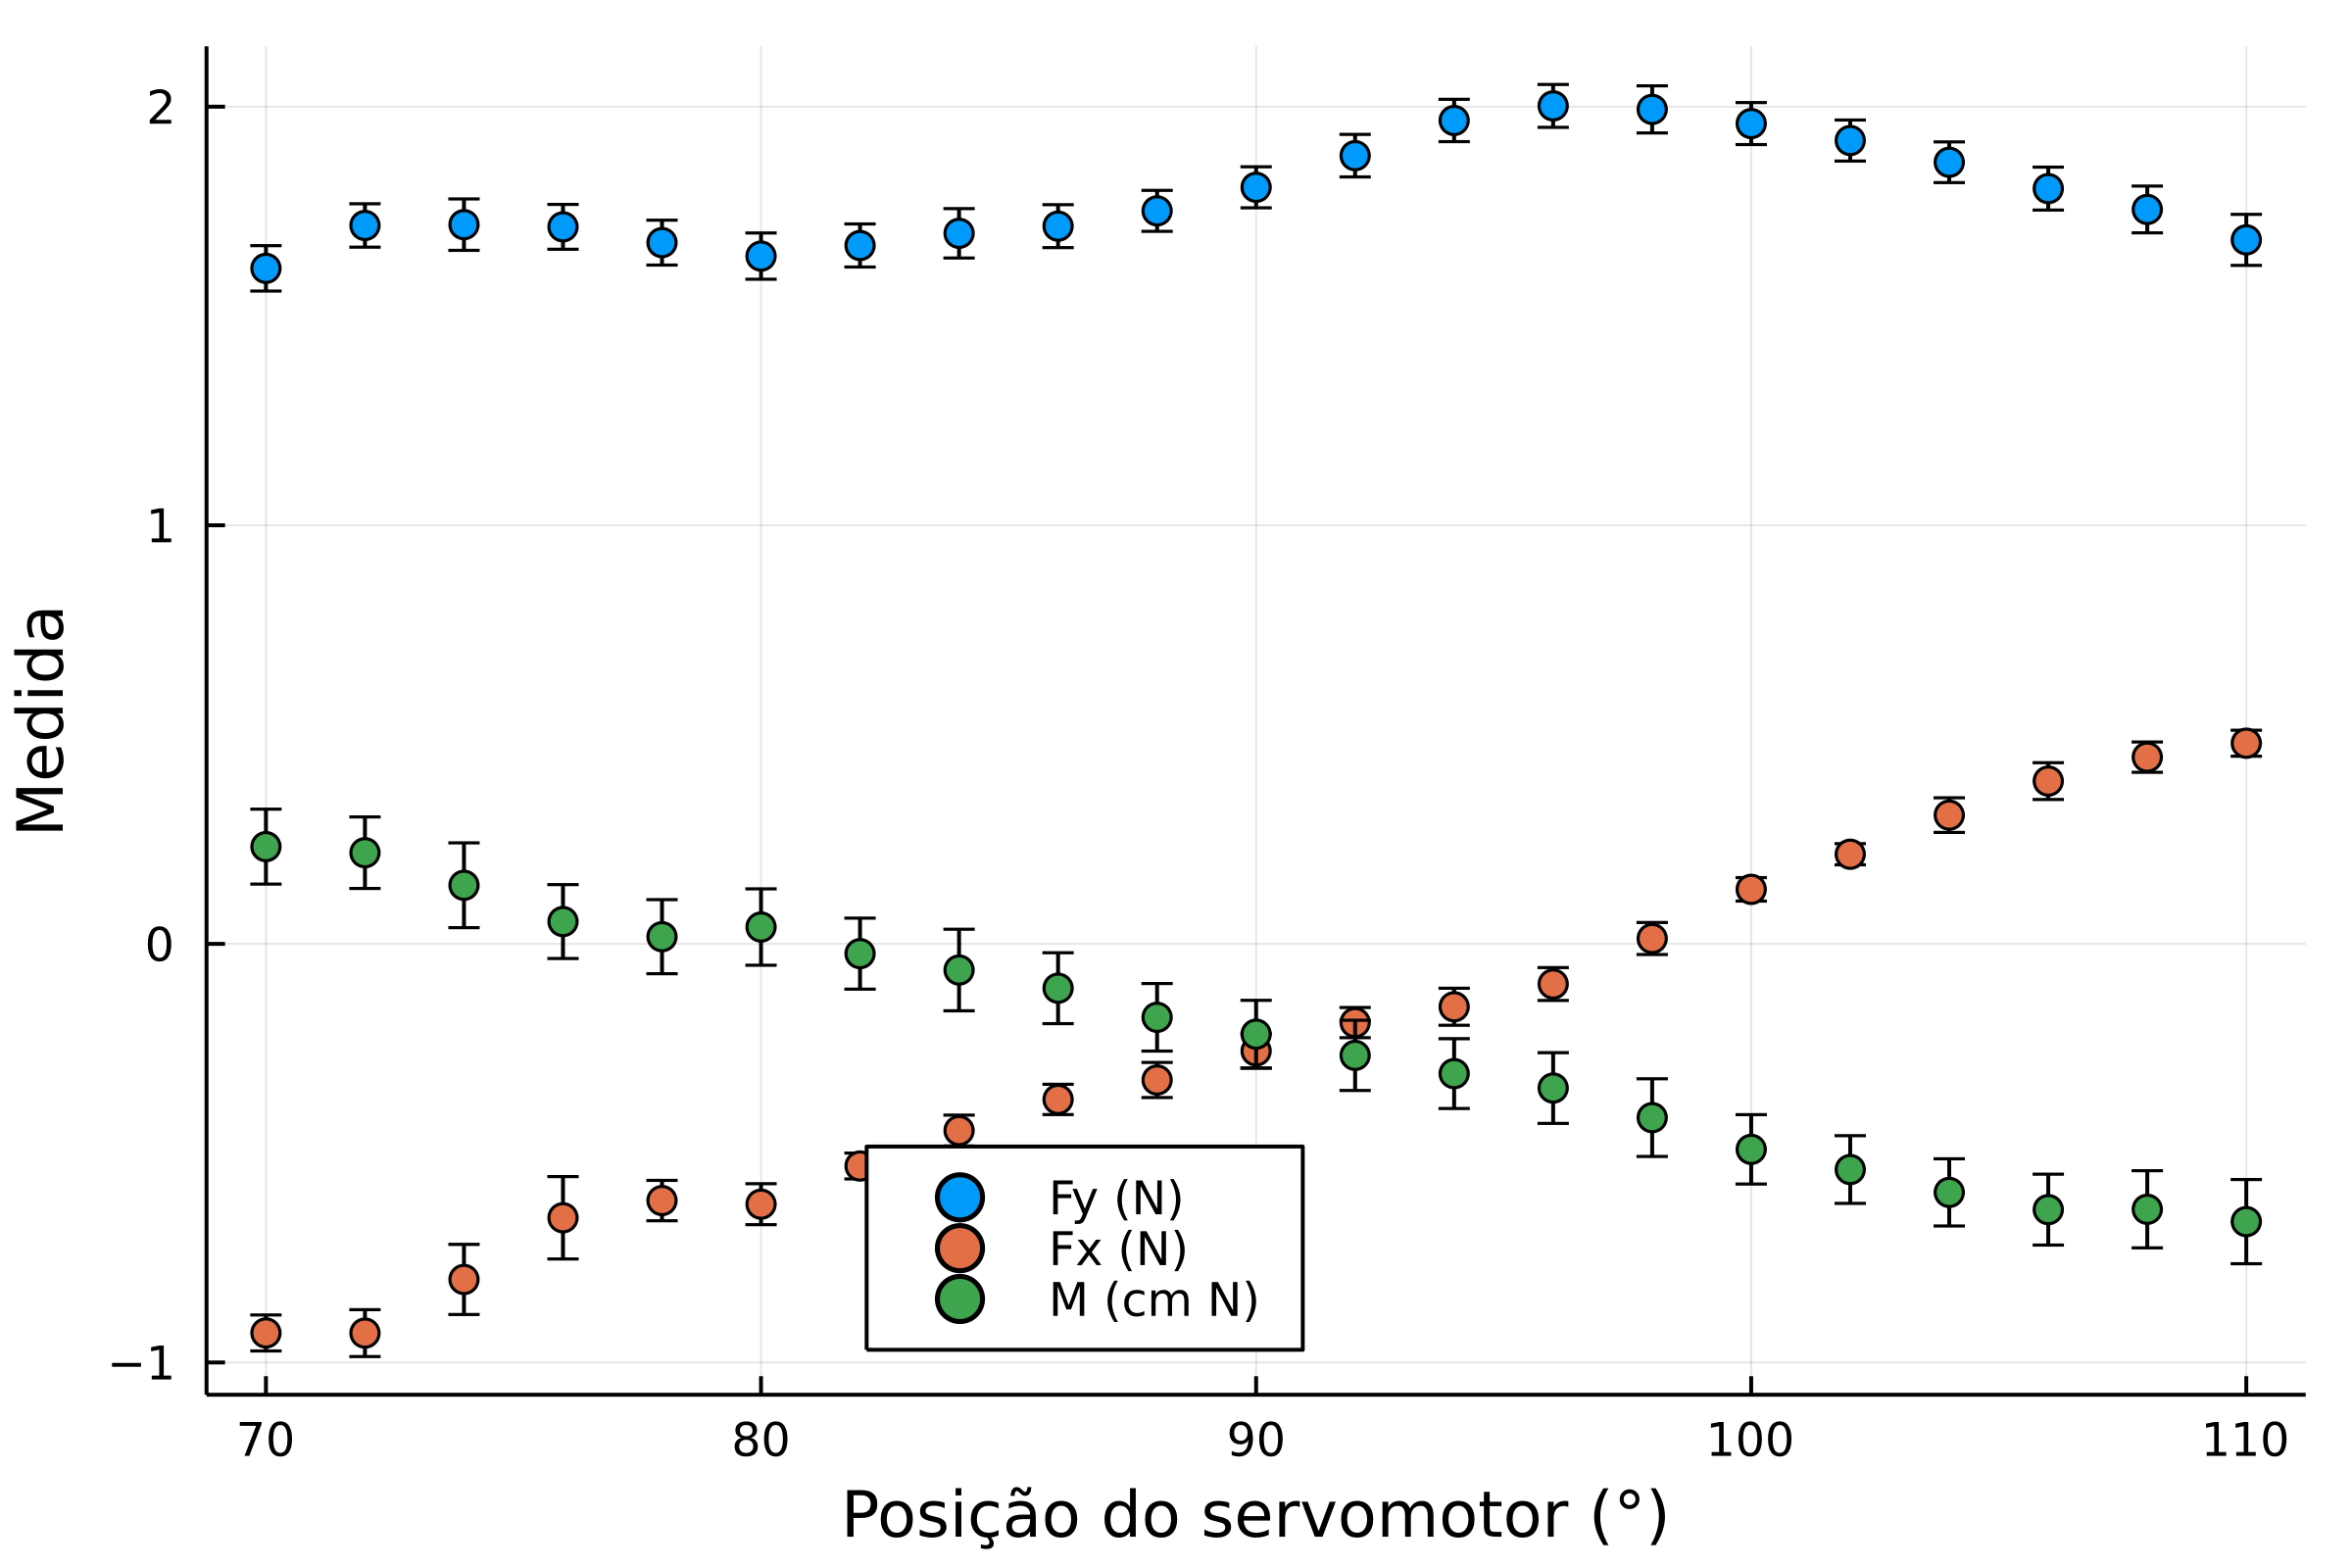
\includegraphics[width=\textwidth]{img/results/exp11_5bar_70_a_110.png}
    \end{subfigure}
    \begin{subfigure}{0.49\textwidth}
        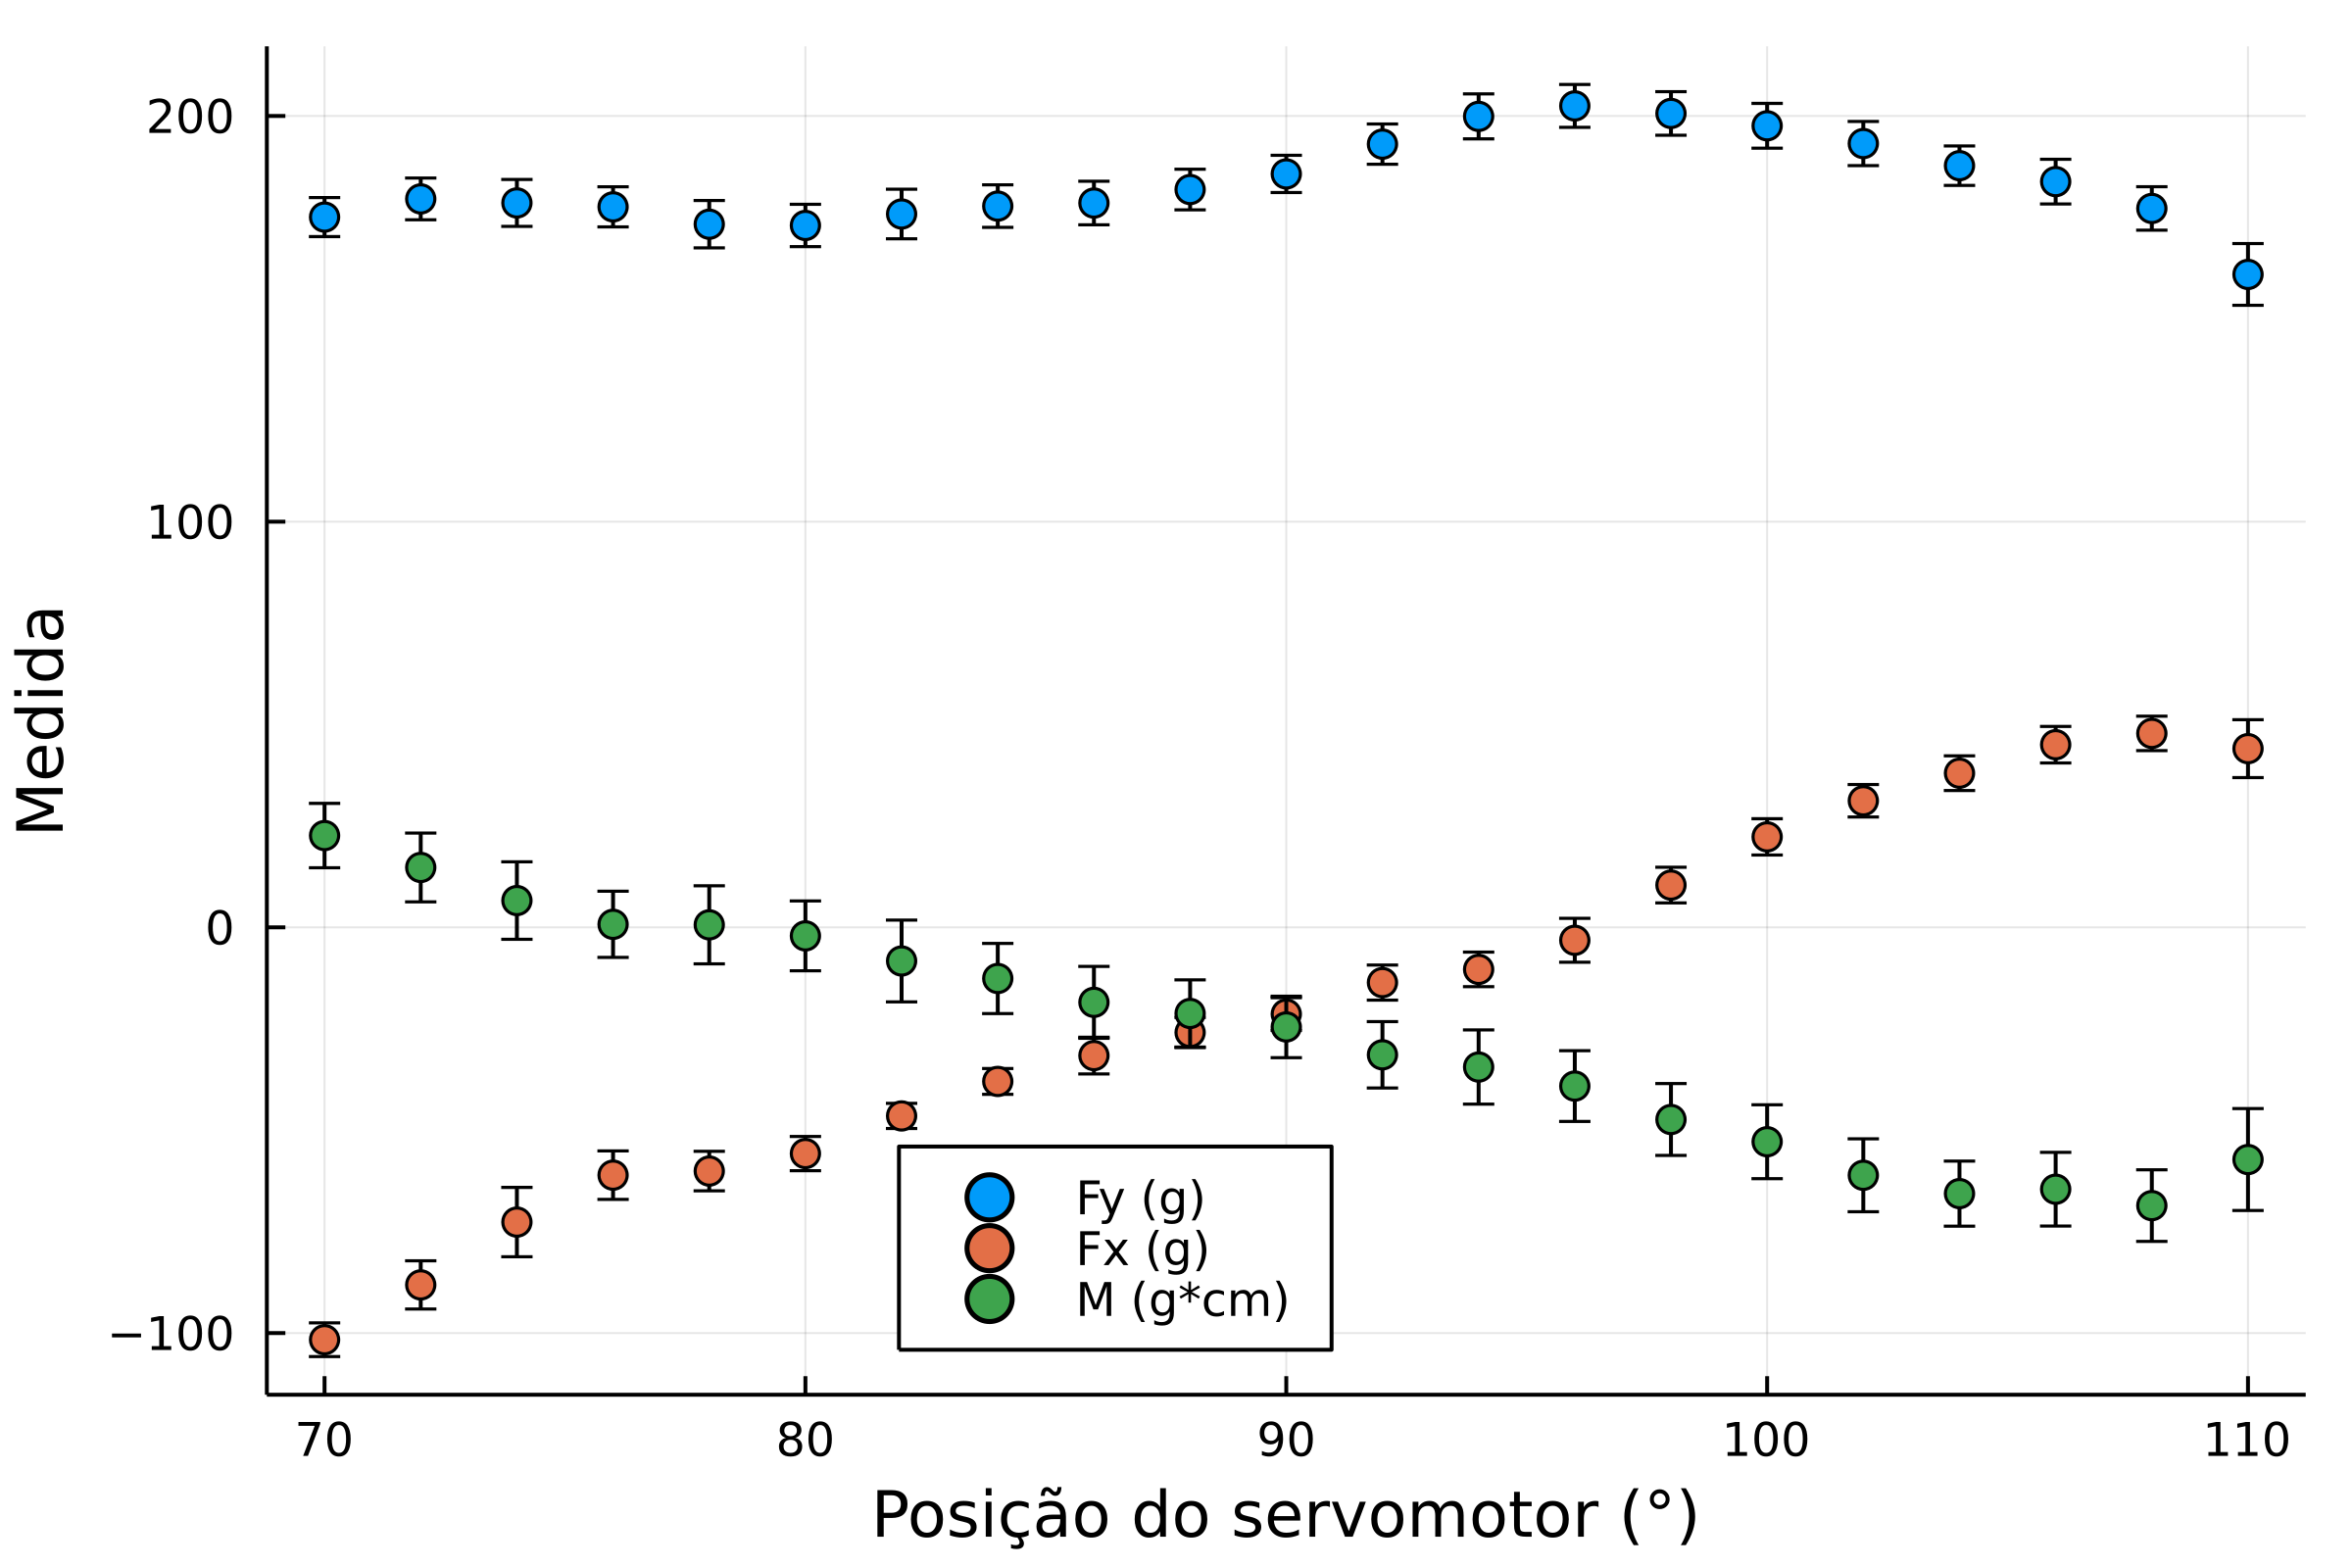
\includegraphics[width=\textwidth]{img/results/exp12_5bar_110_a_70.png}
    \end{subfigure}
    \caption{Curvas de força longitudinal, força transversal e momento medidas para as varreduras de deflexão.}\label{fig:deflection_forces}
\end{figure}

Os gráficos à esquerda correspondem às varreduras no sentido \(70\mathrm{^{\circ}} \rightarrow 110\mathrm{^\circ}\) e os à direita, às varreduras no sentido contrário. Se houvesse folga mecânica nos componentes, seria esperado haver discordância entre os gráficos da esquerda e da direita, devido à mudança de sentido da força sofrida pelo sistema defletor ao passar pela posição \(90\mathrm{^{\circ}}\). Havendo, pelo contrário, forte semelhança entre os gráficos, é possível excluir imperfeições mecânicas como fonte de erros para o sistema. Observa-se aqui que o momento apresentado nos gráficos refere-se ao momento ao redor do eixo da balança (localizado nas figuras~\ref{fig:jet_vanes_assembly_side},~\ref{fig:jet_vanes_render1} e~\ref{fig:montagem_interna}).

As curvas de força transversal e momento apresentam comportamento linear para pequenas deflexões. Observa-se, em todos os gráficos, uma mudança no coeficiente angular destas quantidades por volta dos \(115\mathrm{^{\circ}}\), o que corresponde ao término da região linear prevista pela equação~\ref{eq:sslift}. Nota-se no entanto que na posição \(90\mathrm{^\circ}\) há forças e momentos residuais, o que não condiz com a simetria esperada para a configuração. Esta assimetria pode ser atribuída a erros experimentais introduzidos pelo equipamento, como por exemplo a rigidez da mangueira de gás, alterada pelo escoamento a alta pressão em seu interior, como discutido na seção~\ref{sec:method_3axis_measurement}. Observa-se também que devido ao corte da lâmina defletora com tesouras de metal, seu perfil também é um pouco assimétrico. O fato destes valores serem semelhantes para todos os experimentos conduzidos corrobora a hipótese de que são fruto de erros experimentais sistemáticos e podem, portanto, ser desconsiderados.

Quanto à curva de força longitudinal ou empuxo, \(F_y\), percebe-se que houve uma redução consistente de empuxo em relação ao empuxo sem lâmina defletora da figura~\ref{fig:thrust_no_deflector}. A introdução de uma lâmina de espessura não nula gera ondas de choque no escoamento supersônico mesmo a ângulo de ataque nulo~\cite{anderson}, que reduzem a velocidade do escoamento e portanto o empuxo do motor. Observa-se também um pico de empuxo próximo à deflexão de \(100\mathrm{^\circ}\), correlacionado com o momento durante o experimento no qual o compressor foi reativado devido ao seu esvaziamento. Assim, esta curva apresenta erros experimentais significativos, de modo que quaisquer variações reais de empuxo em função da deflexão da lâmina são indetermináveis.

Tendo sido exibidos os gráficos diretamente obtidos dos dados experimentais, e tendo sido constatada sua semelhança, extrair-se-ão parâmetros médios para o sistema. O empuxo médio obtido foi 
\begin{equation}
    F_{av} = 1,77 \pm 0,02\;\mathrm{N}
\end{equation}
correspondendo a uma redução de 41\% em relação ao empuxo sem lâmina defletora, o que leva a considerações de projeto importantes em relação à eficiência. É possível também calcular derivadas de controle médias para a força transversal e para o momento:
\begin{align}
    F_{x\delta} &= (3,57 \pm 0,05)\times10^{-2} \mathrm{N} / \mathrm{^\circ} \\
    M_\delta &= (-2,29 \pm 0,02)\times10^{-2} \mathrm{N}\,\mathrm{cm} / \mathrm{^\circ}
\end{align}
onde \(\delta \) representa a deflexão da lâmina. O momento é dado em relação ao eixo da balança.\ 

\section{Discussão sobre a metodologia}

O estudo sobre vetorização de empuxo é uma área promissora mas nova no Brasil. Desta forma, este trabalho foi uma primeira aproximação do assunto, no qual foram feitas suposições sobre a metodologia adequada para estudar o tema. Agora, avaliar-se-ão algumas das escolhas feitas, considerando a possibilidade de trabalhos futuros.

A escolha do gás frio como propelente deve-se à sua temperatura, que permite o uso de componentes impressos em 3D, bem como à sua disponibilidade e custo. Outra característica do gás frio constatada no trabalho é sua reprodutibilidade: o empuxo é estável (figura~\ref{fig:thrust_no_deflector}) e não varia entre ativações do motor (figura~\ref{fig:deflection_forces}). Todas essas são características desejáveis e provaram-se necessárias para a execução do trabalho. Supondo, por exemplo, que o trabalho tivesse sido conduzido com um motor de combustível sólido, introduzir-se-iam variações devido à mistura dos propelentes e devido à curva de empuxo do motor~\cite{Sutton}, além de introduzir-se a necessidade de manufaturar todos os componentes em materiais resistentes à temperatura. Estima-se que o motor tenha sido ativado por cerca de \(20\mathrm{min}\) ao longo do trabalho, de modo que seria necessário fabricar vários grãos-propelente para a execução dos testes necessários.

No entanto, a baixa energia do propelente significa que uma alta vazão mássica é necessária mesmo para os pequenos empuxos usados no trabalho. Originalmente almejava-se usar um motor de \(5\mathrm{N}\), mas este provou-se inviável devido à velocidade de consumo de ar comprimido. Ao longo do projeto foram utilizados cilindros de nitrogênio comprimido e dois compressores de ar distintos (40L e 8bar e 400L e 9bar). O cilindro de nitrogênio, de \(200\mathrm{bar}\) e 50L foi esvaziado rapidamente, e o primeiro compressor apresentava uma rápida queda de pressão (motivo pelo qual o gráfico~\ref{fig:thrust_no_deflector} apresenta pressão variável). O maior compressor durou mais tempo, mas possivelmente introduziu erros nos gráficos da~\ref{fig:deflection_forces}. Dessa forma, para trabalhos futuros, garantir a compatibilidade do sistema propulsivo com o sistema de fornecimento de ar comprimido é fundamental.\ 

Quanto à balança de três componentes usada, faz-se necessário encontrar alternativas para trabalhos futuros. A balança é montada a um túnel de vento, o que restringe a montagem do sistema propulsivo. Isto impediu, por exemplo, a montagem de um transdutor de pressão na câmara de empuxo nas medidas finais, já que essa montagem introduziria ainda mais erros devidos à rigidez da mangueira. Tendo sido adquirida para medir forças da escala de 5 a 20N~\cite{lab}, ela mostra-se inadequada para as forças permitidas pelos sistemas de fornecimento de ar comprimido disponíveis. Este aparato não é de simples fabricação, sendo necessária precisão micrométrica para alguns componentes. No entanto, parece ser um passo necessário para o desenvolvimento de sistemas de vetorização de empuxo no Brasil a fabricação de uma bancada de teste de empuxo com balança de três componentes (para sistemas com um grau de liberdade, que geram forças e momento em um plano) ou seis componentes (para medição completa de forças e momentos tridimensionais), específicas para o propósito.\

Por fim, discutem-se questões relacionadas diretamente ao sistema de vetorização e à lâmina defletora. A tabela~\ref{tab:proj_params} apresenta uma relação de novos parâmetros de projeto introduzidos pela adição do sistema de vetorização a um sistema propulsivo, bem como os \textit{trade-offs} de engenharia que os acompanham.

\begin{table}[htbp]
    \centering\begin{tabular}{p{.3\linewidth}p{.3\linewidth}p{.3\linewidth}} \toprule
        Parâmetro & \textit{Trade-off} associado & Critério de escolha para este trabalho \\[.3cm] \midrule
        Espessura da lâmina & Perda de empuxo contra ganho de integridade estrutural & Disponibilidade de material e rigidez ao manuseio  \\[.3cm]
        Distância da tubeira à lâmina & Perda de empuxo contra ganho de derivadas de controle & Espaço para montagem\\[.3cm]
        Corda da lâmina & Ganho de derivadas de controle contra aumento do momento aerodinâmico sobre a lâmina & Escala próxima aos componentes já escolhidos\\[.3cm]
        Posição do eixo em relação ao bordo de ataque da lâmina defletora & Exigência de torque do atuador contra integridade estrutural & Centro\\[.3cm]
        Resolução e torque máximo do atuador & Capacidades contra custo & Disponibilidade, tamanho \\ \bottomrule
    \end{tabular}
    \caption{Parâmetros de projeto referentes ao sistema de vetorização de empuxo.}\label{tab:proj_params}
\end{table}

A grande perda de empuxo observada com a inserção da lâmina defletora pode ser atribuída ao fato de que a espessura da lâmina, \(0,7\,\mathrm{mm}\) é 58\% do diâmetro da tubeira, \(1,2\,\mathrm{mm}\). A influência da distância da tubeira à lâmina deve ser examinada em um trabalho futuro, pois esta grandeza foi constante neste trabalho (cerca de \(1\,\mathrm{cm}\)). A corda da lâmina também foi mantida constante em \(1,1\,\mathrm{cm}\). Posicionar o eixo na metade da corda da lâmina é uma decisão que se justifica pela previsão de que para placas infinitamente planas em escoamentos uniformes, como a situação da figura~\ref{fig:supersonic_flat_plate}, o ponto neutro situa-se neste ponto~\cite{anderson}. Destaca-se também que a lâmina pode sofrer \textit{flutter}~\cite{flutter}, o que pode ser mitigado por engastes adequados no eixo. Por fim, foi introduzido um componente eletromecânico ao sistema propulsivo, o servomotor, que apresenta limites de resolução e torque máximo. Historicamente, o atuador foi geralmente eletro-hidráulico, mas há um interesse recente em realizar sistemas eletromecânicos de vetorização de empuxo~\cite{etvc}.

% REFERENCIAS BIBLIOGRAFICAS
\renewcommand\bibname{\itareferencesnamebabel} %renomear título do capítulo referências
\bibliography{Referencias/referencias}

% Apendices
\appendix

% Anexos
\annex

% Glossario
%\itaglossary
%\printglossary

% Folha de Registro do Documento
% Valores dos campos do formulario
\FRDitadata{25 de março de 2015}
\FRDitadocnro{DCTA/ITA/DM-018/2015} %(o número de registro você solicita a biblioteca)
\FRDitaorgaointerno{Instituto Tecnológico de Aeronáutica -- ITA}
%Exemplo no caso de pós-graduação: Instituto Tecnol{\'o}gico de Aeron{\'a}utica -- ITA
\FRDitapalavrasautor{Cupim; Cimento; Estruturas}
\FRDitapalavrasresult{Cupim; Dilema; Construção}
%Exemplo no caso de graduação (TG):
%\FRDitapalavraapresentacao{Trabalho de Graduação, ITA, São José dos Campos, 2015. \NumPenultimaPagina\ páginas.}
%Exemplo no caso de pós-graduação (msc, dsc):
\FRDitapalavraapresentacao{ITA, São José dos Campos. Curso de Mestrado. Programa de Pós-Graduação em Engenharia Aeronáutica e Mecânica. Área de Sistemas Aeroespaciais e Mecatrônica. Orientador: Prof.~Dr. Adalberto Santos Dupont. Coorientadora: Prof$^\textnormal{a}$.~Dr$^\textnormal{a}$. Doralice Serra. Defesa em 05/03/2015. Publicada em 25/03/2015.}
\FRDitaresumo{Aqui começa o resumo do referido trabalho. Não tenho a menor idéia do que colocar aqui. Sendo assim, vou inventar. Lá vai: Este trabalho apresenta uma metodologia de controle de posição das juntas passivas de um manipulador subatuado de uma maneira subótima. O termo subatuado se refere ao fato de que nem todas as juntas ou graus de liberdade do sistema são equipados com atuadores, o que ocorre na prática devido a falhas ou como resultado de projeto. As juntas passivas de manipuladores desse tipo são indiretamente controladas pelo movimento das juntas ativas usando as características de acoplamento da dinâmica de manipuladores. A utilização de redundância de atuação das juntas ativas permite a minimização de alguns critérios, como consumo de energia, por exemplo.
Apesar da estrutura cinemática de manipuladores subatuados ser idêntica a do totalmente atuado, em geral suas caraterísticas dinâmicas diferem devido a presença de juntas passivas. Assim, apresentamos a modelagem dinâmica de um manipulador subatuado e o conceito de índice de acoplamento. Este índice é utilizado na sequência de controle ótimo do \mbox{manipulador}.
A hipótese de que o número de juntas ativas seja maior que o número de
passivas  $(n_{a} > n_{p})$  permite o controle ótimo das juntas passivas, uma vez que na etapa de controle destas há mais entradas (torques nos atuadores das juntas ativas), que elementos a controlar (posição das juntas passivas). }
%  Primeiro Parametro: Nacional ou Internacional -- N/I
%  Segundo parametro: Ostensivo, Reservado, Confidencial ou Secreto -- O/R/C/S
\FRDitaOpcoes{N}{O}
% Cria o formulario
\itaFRD

\end{document}
% Fim do Documento. O massacre acabou!!! :-)
